\newcommand{\econtexRoot}{.}
% The \commands below are required to allow sharing of the same base code via Github between TeXLive on a local machine and ShareLaTeX.  This is an ugly solution to the requirement that custom LaTeX packages be accessible, and that ShareLaTeX seems to ignore symbolic links (even if they are relative links to valid locations)
\providecommand{\econtex}{\econtexRoot/texmf-local/tex/latex/econtex}
\providecommand{\econtexSetup}{\econtexRoot/texmf-local/tex/latex/econtexSetup}
\providecommand{\econtexShortcuts}{\econtexRoot/texmf-local/tex/latex/econtexShortcuts}
\providecommand{\econtexBibMake}{\econtexRoot/texmf-local/tex/latex/econtexBibMake}
\providecommand{\econtexBibStyle}{\econtexRoot/texmf-local/bibtex/bst/econtex}
\providecommand{\notes}{\econtexRoot/texmf-local/tex/latex/handout}
\providecommand{\handoutSetup}{\econtexRoot/texmf-local/tex/latex/handoutSetup}
\providecommand{\handoutShortcuts}{\econtexRoot/texmf-local/tex/latex/handoutShortcuts}
\providecommand{\handoutBibMake}{\econtexRoot/texmf-local/tex/latex/handoutBibMake}
\providecommand{\handoutBibStyle}{\econtexRoot/texmf-local/bibtex/bst/handout}

  

\documentclass{beamer}
\usepackage{remreset}
\usepackage{etoolbox}
\usepackage{comment}
\usepackage{graphicx}
%\usepackage{dtklogos}
\usepackage{dsfont}
\usepackage{amsmath,amssymb}
\usepackage{econtexShortcuts}
\usepackage[english]{babel}
\usepackage{tikz} 
\usepackage{cancel}
\usepackage{booktabs,natbib}
\setbeamercovered{invisible}

\usepackage{dcolumn}


\makeatletter
\@removefromreset{subsection}{section}
\patchcmd{\beamer@part}{\setcounter{subsection}{0}}{}{}
\makeatother
\setcounter{subsection}{1}
\setbeamercovered{transparent}

\mode<presentation>{}
%% preamble
\title[Consumption Heterogeneity: Micro Drivers and Macro Implications]{Consumption Heterogeneity: \\ Micro Drivers and Macro Implications}
\author{Edmund Crawley \& Andreas Kuchler}
\date[8/6/2018]{Federal Reserve Board, August 6, 2018}
\usetheme{Frankfurt}
\begin{document}
\newcolumntype{d}[1]{D{.}{.}{#1}}
%circled draws a circle around a number
\newcommand*\circled[1]{\tikz[baseline=(char.base)]{
		\node[shape=circle,draw,inner sep=2pt] (char) {#1};}}


\frame{\titlepage}
\section{Motivation}
\setbeamercovered{invisible}
\frame
{
	\frametitle{Overview}
	What will this paper do?\\
	\begin{itemize}	
	\item[1] Create a new method to estimate heterogeneity in consumption responses to permanent and transitory shocks to income
	\begin{itemize}
		\item Clear negative relation between MPC and liquid wealth
	\end{itemize}
	\item[2] Application: Redistribution Channel of Monetary Policy (\cite{auclert_monetary_2017})
	\begin{itemize}
		\item We find a transitory 1\% interest rate rise decreases consumption by 0.33\% through the interest rate exposure channel
		\item This channel is likely far larger than the intertemporal substitution channel (1-6x as large)
	\end{itemize}
	\end{itemize}	
}
\frame{
	\frametitle{How Are Consumption Responses Typically Measured?}
	Three methods:
	\begin{itemize}
		\item[1] (Natural) Experiments - stimulus checks, lotteries etc
		\begin{itemize}
			\item Few true experiments, especially for permanent shocks
			\item Data limitations
		\end{itemize}
		\item[2] Ask people
		\begin{itemize}
			\item Unclear how to interpret
		\end{itemize}
		\item[3] Use covariance structure of income and consumption
		\begin{itemize}
			\item Empirical methods (until now!) have been flawed
		\end{itemize}
	\end{itemize}
	\bigskip
	We develop a robust method based on 3
}
\frame
{
	\frametitle{Evidence on Magnitude of Consumption Response}
	\resizebox{\textwidth}{!}{
	\centering
		\input ../Tables/MPCLiterature.tex }
	\tiny{$^{\star}$ Elasticity \\
		 Methods 1) Natural Experiment 2) Survey question 3) Covariance restrictions} \\
    Table mostly lifted from \cite{carroll_distribution_2017}
}

\frame
{
	\frametitle{Evidence on Distribution of Consumption Response}
	Most studies do not have enough power to say anything about how their MPC estimates vary in the population\\
	\bigskip
	Exceptions:
	\begin{itemize}
		\item \cite{jappelli_fiscal_2014} Italian Survey Data
		\item \cite{fagereng_mpc_2016} Norway Lottery Data
		\item \cite{gelman_what_2016} Financial App Data
		\item \cite{fuster_what_2018} NY Fed Survey
	\end{itemize}
	\bigskip
	\textbf{Liquid assets} and \textbf{income} are key predictors of transitory MPC
}

\frame
{
	\frametitle{Application: \cite{auclert_monetary_2017}}
	\cite{auclert_monetary_2017} identifies three ways in which \textbf{heterogeneity} affects monetary policy\\
	Each is potentially measurable in panel data\\
	But...
	\pause
	\begin{columns}
	\column{0.5\linewidth}
	\centering
	\begin{figure}
	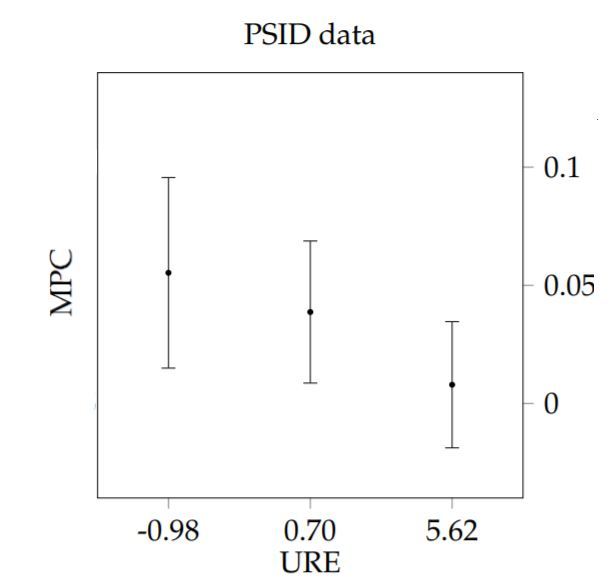
\includegraphics[trim=0 0 0 0,clip,scale=0.5]{../Figures/MPCDistributionAuclert_URE.jpg}
	\end{figure}
	He doesn't have the right data or methods to be able to do this
	\pause
	\column{0.5\linewidth}
	\centering
	\begin{figure}
	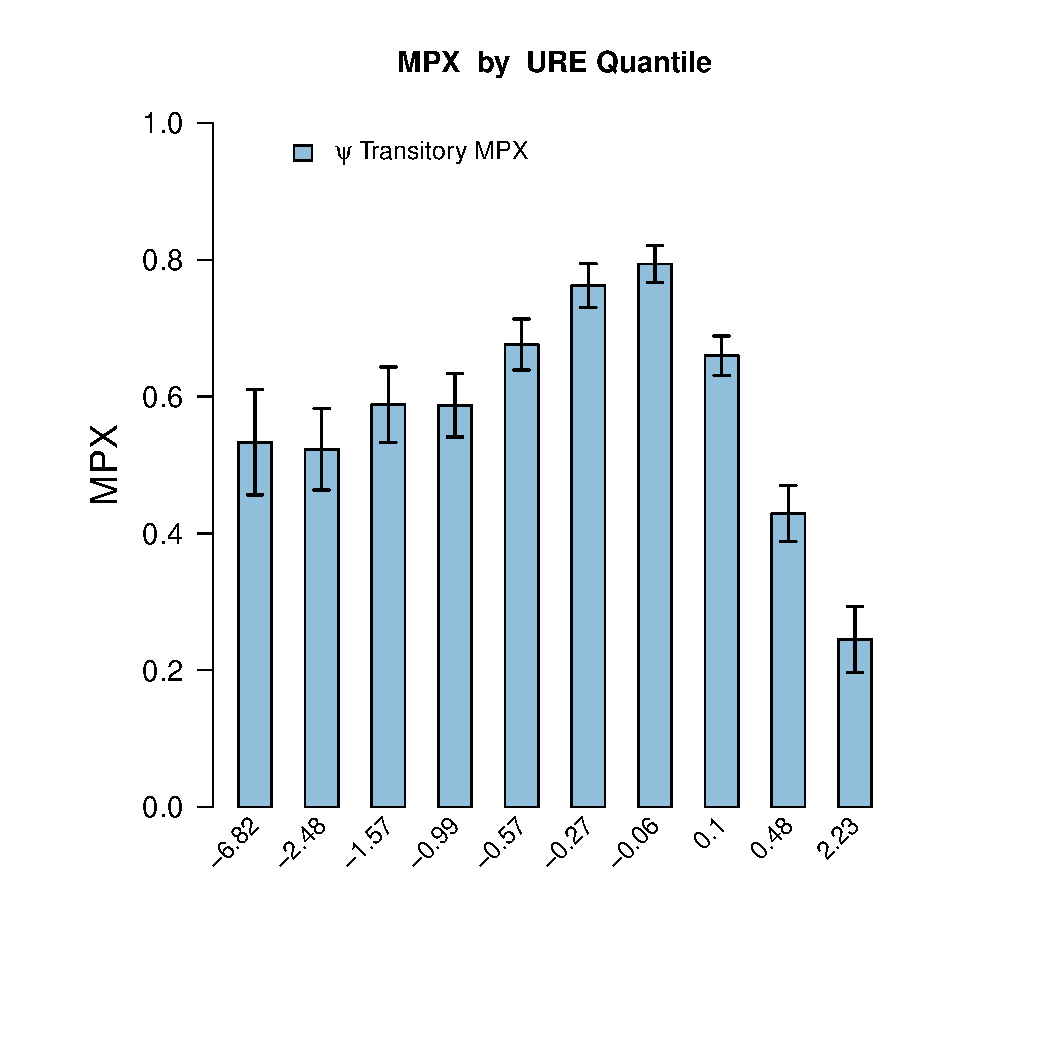
\includegraphics[trim= 0 3.2cm 0 1.8cm, clip, scale=0.25]{../Figures/MPXByURE_level_lincome_head.pdf}
	\end{figure}
	We can do a lot better!
	\end{columns}
}
\section{Empirical Strategy}
\setbeamercovered{invisible}
\frame
{
	\frametitle{Methodology Intuition}
	Exploit increasing importance of permanent shocks as the time over which growth is measured increases
	\begin{columns}
	\column{0.6\linewidth}
	\centering
	\begin{tikzpicture}
	\node (img1) {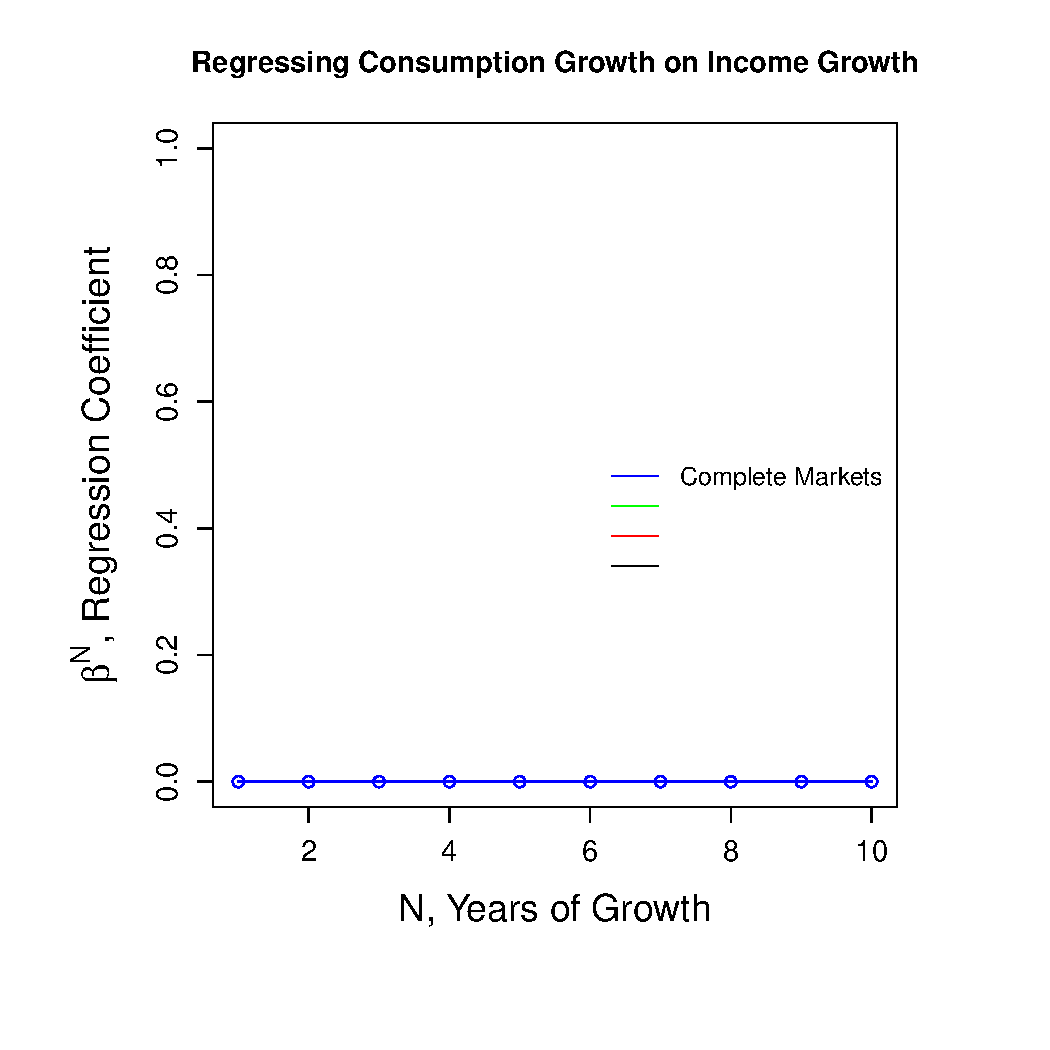
\includegraphics[height=6.5cm]{../Figures/basic_regression_complete_level_lincome_head.pdf}};
	\pause
	\node (img2) {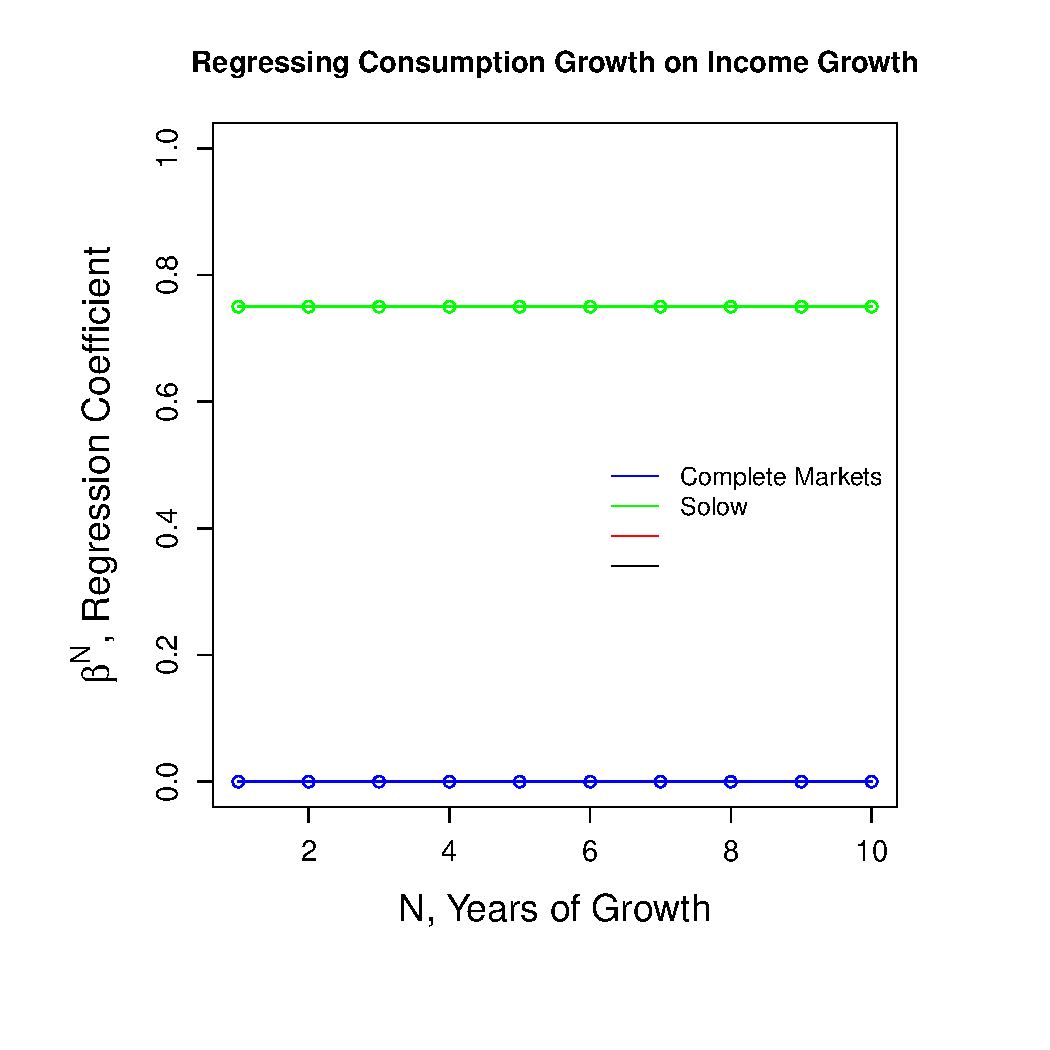
\includegraphics[height=6.5cm]{../Figures/basic_regression_solow_level_lincome_head.pdf}};
	\pause
	\node (img3) {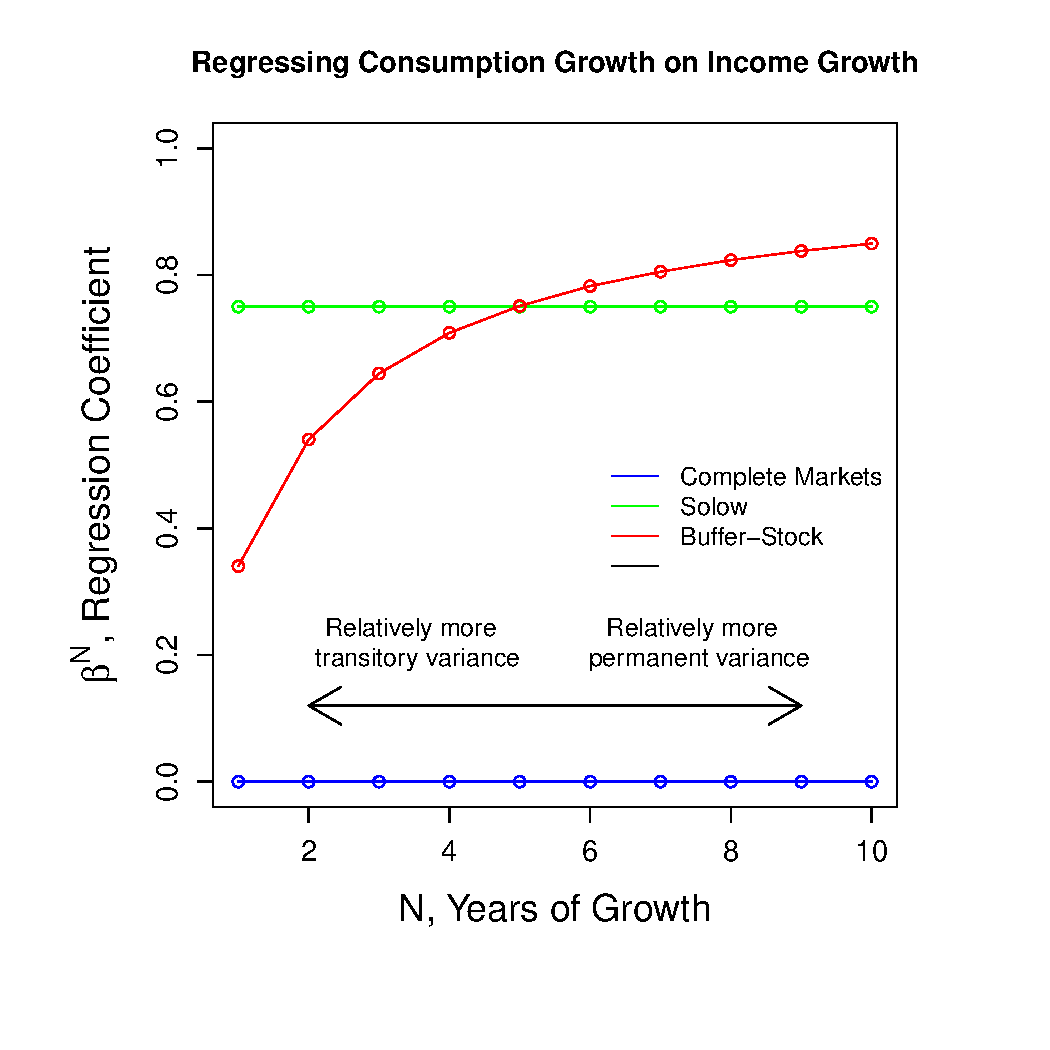
\includegraphics[height=6.5cm]{../Figures/basic_regression_BS_level_lincome_head.pdf}};
	\pause
	\node (img4) {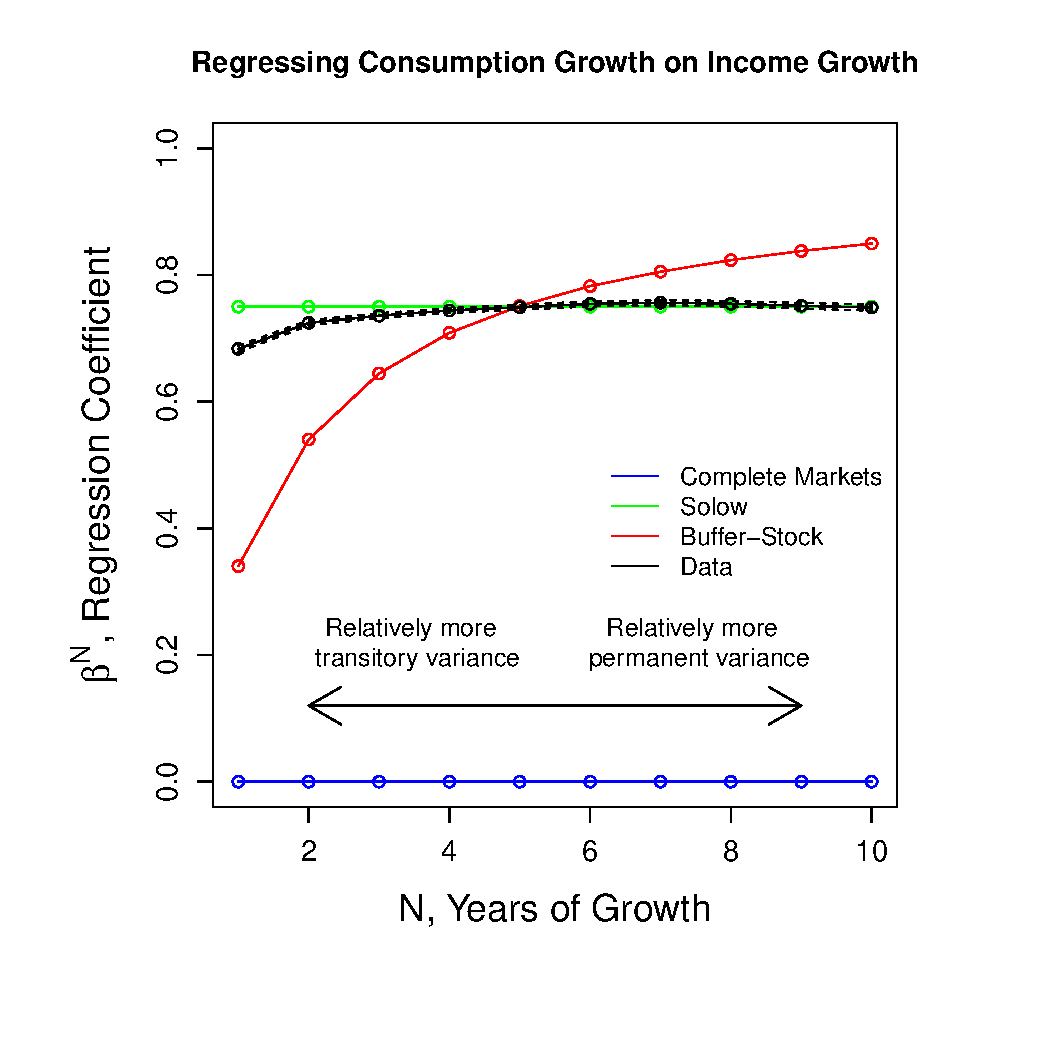
\includegraphics[height=6.5cm]{../Figures/basic_regression_level_lincome_head.pdf}};
	\pause
	\node (img5) {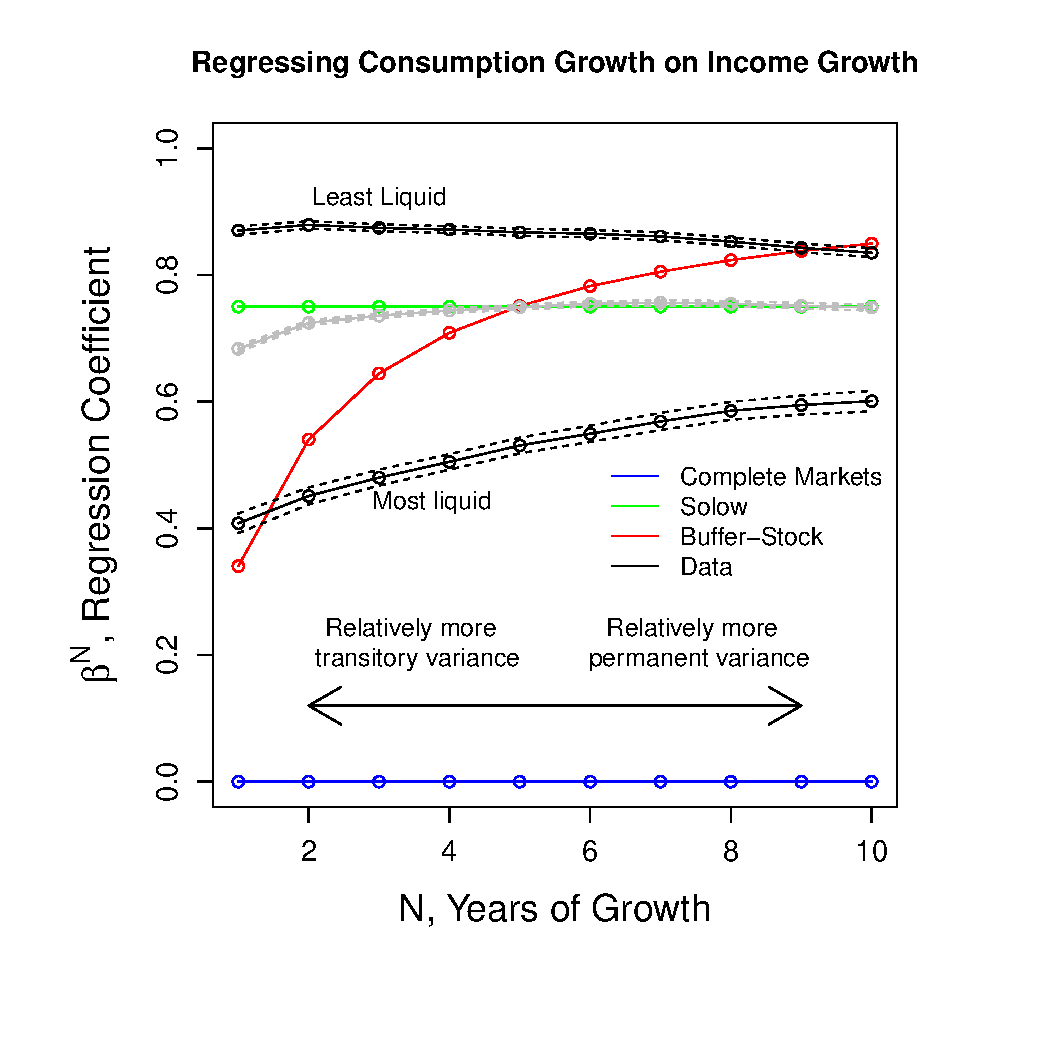
\includegraphics[height=6.5cm]{../Figures/basic_regression_liquid_wealth_level_lincome_head.pdf}};
	\end{tikzpicture}
	\column{0.4\linewidth}
	\begin{align*}
	\Delta^N c_i = \beta^N \Delta^N y_i +\varepsilon_i
	\end{align*}
	\end{columns}

}
\frame
{
	\frametitle{Aside: Why Not Blundell, Pistaferri and Preston 2008?}
	1) Time Aggregation Problem (Crawley 2018)
	\begin{columns}
	\column{0.5\linewidth}
	\centering
	\onslide<1->{
	\begin{tikzpicture}
	\node (img1) {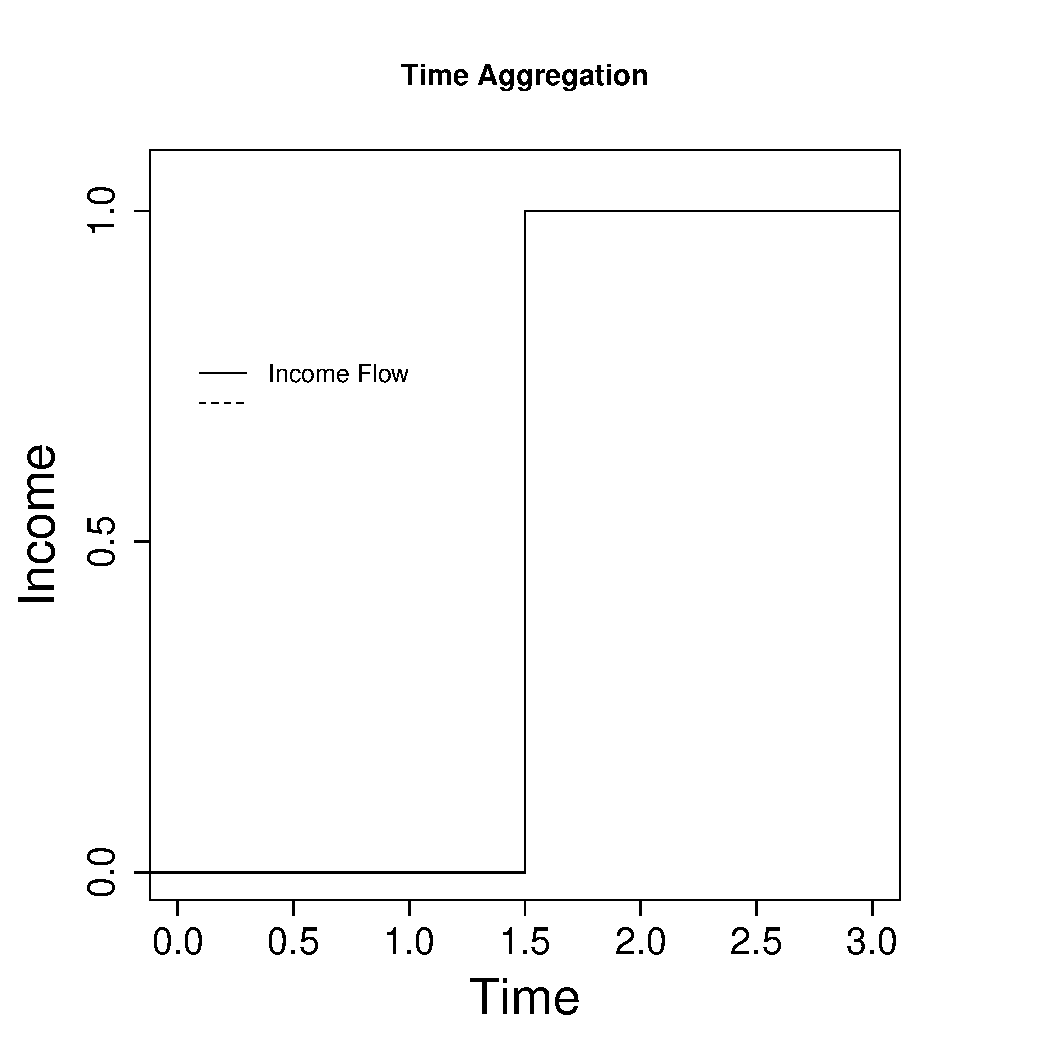
\includegraphics[height=5cm]{../Figures/TimeAggExample1.pdf}};
	\onslide<2->{
	\node (img2) {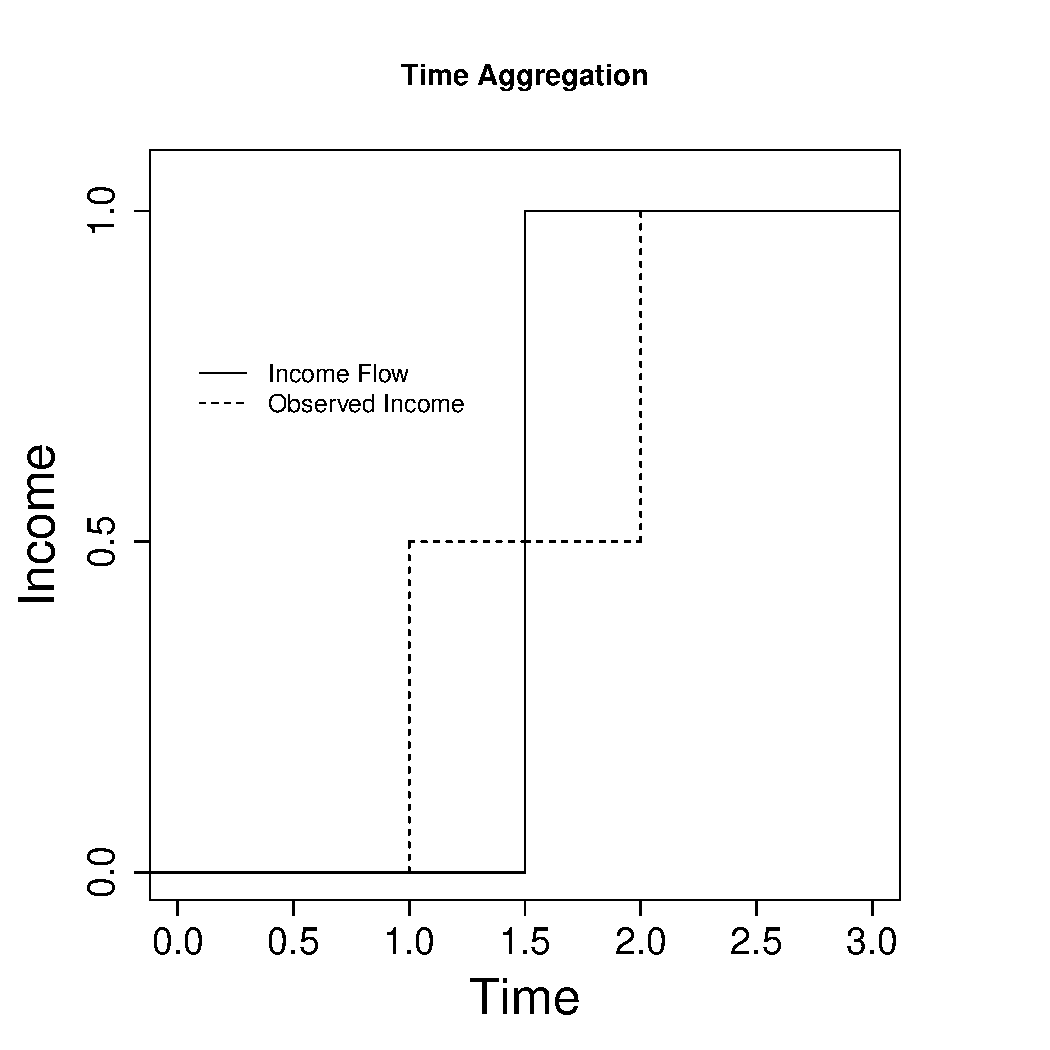
\includegraphics[height=5cm]{../Figures/TimeAggExample2.pdf}};
	}
	\end{tikzpicture}
	}
	\column{0.5\linewidth}
	\onslide<3->{
	PIH Example:\\
	\begin{itemize}
	\item MPC out of Permanent Shocks = 1\\
	\item MPC out of Transitory Shocks = 0\\
	\end{itemize}
	BPP method estimates MPC out of transitory shocks to be -0.6
	\end{columns}
	}
}
\frame
{
	\frametitle{Aside: Why Not Blundell, Pistaferri and Preston 2008?}
	2) BPP assume consumption is a random walk
	\begin{itemize}
		\item High transitory MPCs are incompatible with consumption following a random walk
	\end{itemize}
}
\frame
{
	\frametitle{Identification of the Income Process}
	We follow the spirit of Carroll \& Samwick (1997):\\
	\begin{itemize}
		\item Permanent income follows a random walk
		\begin{align*}
			p_t = p_{t-1} + \zeta_t
		\end{align*}
		\item Total income includes a transitory component
		\begin{align*}
			y_t = p_t +\varepsilon_t
		\end{align*}
	\end{itemize}
	Growth over N years is:
	\begin{align*}
	\Delta^N y_T &=  (\zeta_{T-N+1} + ... +\zeta_T) + \varepsilon_T - \varepsilon_{T-N} \\
	\mathrm{Var}(\Delta^N y_T) &= N\mathrm{Var}(\zeta) + 2\mathrm{Var}(\varepsilon)
	\end{align*}
}
\frame
{
	\frametitle{Identification of the Income Process}
	We follow the spirit of Carroll \& Samwick (1997):\\
	\begin{itemize}
		\item If transitory income follows an MA(2) process:
		\begin{align*}
			y_t &= p_t + \varepsilon_t + \theta_1 \varepsilon_{t-1} +\theta_2 \varepsilon_{t-2} \\
			\implies \mathrm{Var}(\Delta^N y_T) &= N\underbrace{\mathrm{Var}(\zeta)}_{\text{Perm var}} + 2\underbrace{(1+\theta_1^2+\theta_2^2)\mathrm{Var}(\varepsilon)}_{\text{``Total" trans var}} \text{ if } N\geq 3
		\end{align*}
	\end{itemize}
	Carroll \& Samwick use $N=3,4,5$ to identify permanent shock variance and ``total" transitory shock variance
	\bigskip
	\pause
	\begin{itemize}
		\item[1] How does time aggregation affect this identification?
		\item[2] What might the equivalent of ``robust to MA(2) transitory shocks" be in continuous time?
	\end{itemize}
}
\frame
{
	\frametitle{Identification of the Income Process}
	Carroll \& Samwick in Continuous Time with Aggregation\\
	\begin{itemize}
		\item To begin assume no persistence in the transitory shock
		\item $p_t$ and $q_t$ are independent martingale processes with independent increments
		\begin{align*}
			\mathrm{Var}(p_t-p_{t-1}) &= \sigma^2_p \\
			\mathrm{Var}(q_t-q_{t-1}) &= \sigma^2_q
		\end{align*}
		\item Instantaneous income is equal to the flow of permanent income plus the transitory income component
		\begin{align*}
		dy_t = p_t dt + dq_t
		\end{align*}
	\end{itemize}
	\pause
	We observe $\bar{y}_T$, total income over year $T$:
	\begin{align*}
	\bar{y}_T &= \int_{T-1}^{T}p_t dt + q_T - q_{T-1} \\
	\implies  \mathrm{Var}(\Delta^N \bar{y}_T) &= (N-\frac{1}{3})\sigma_p + 2\sigma_q
	\end{align*}
}
\frame
{
	\frametitle{Identification of the Income Process}
	Allow a generic persistence in transitory shock
	\begin{itemize}
		\item Following shock, transitory income flow decays as:
		\begin{align*}
			f(t)  \text{ where } f(t)=0 \text{ if } t>2
		\end{align*}
	\end{itemize}
	\vspace*{-0.15in}
	\begin{figure}
		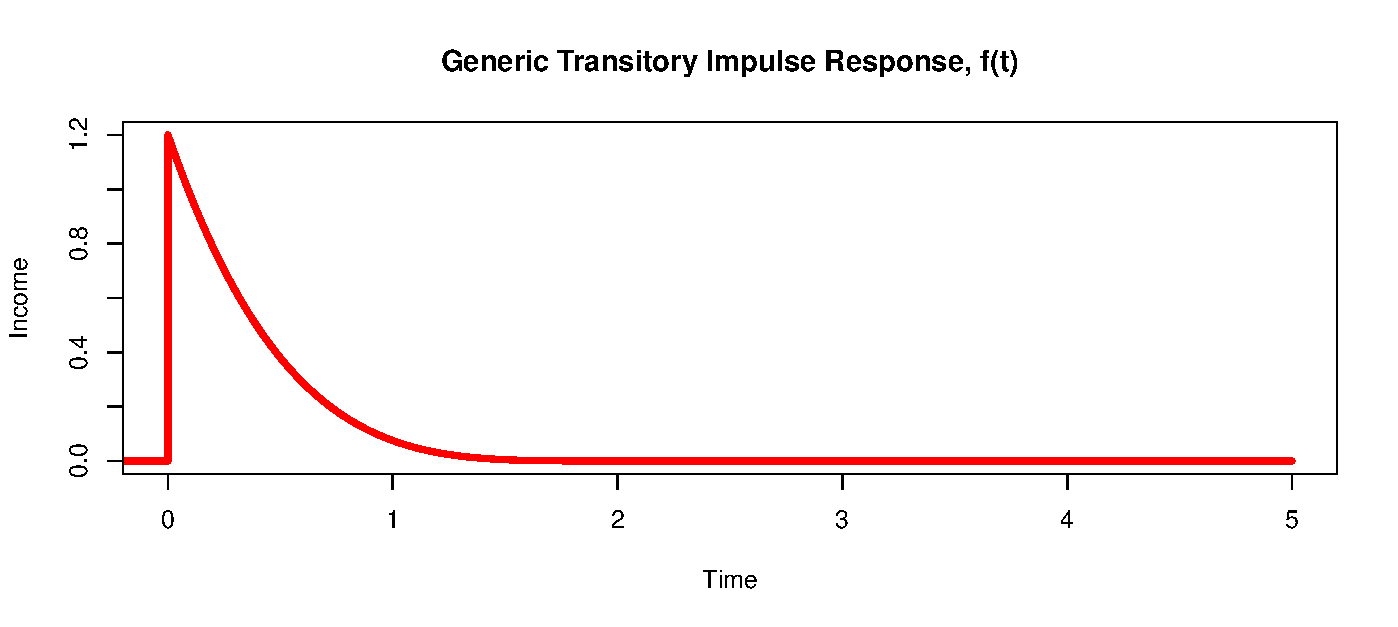
\includegraphics[scale=0.3]{../Figures/GenericTransitory.pdf}
	\end{figure}
	\vspace*{-0.15in}
	\begin{align*}
	y_t &= p_t + \int_{t-2}^{t} f(t-s)dq_s\\
	\implies \mathrm{Var}(\Delta^N \bar{y}_T) &= (N-\frac{1}{3})\sigma^2_p +  2 \sigma^2_{\tilde{q}} \text{   for }N \geq 3
	\end{align*}	
	where $	\tilde{q_T} = \int_{T-1}^{T}\int_{t-2}^{t} f(t-s)dq_s dt$ is the time aggregated transitory component of income
}
\frame
{
	\frametitle{Identification of the Consumption Response}
	\label{cons_identification}
	Assumptions on Consumption\\
	\begin{itemize}
		\item Permanent: Consumption permanently moves by fraction $\phi$ of the income shock
		\item Transitory: Allow for generic impulse response $g(t)$ where $g(t) = 0$ for $t>2$ \qquad \qquad \qquad \qquad \qquad \qquad \qquad \hyperlink{cons_decay}{\beamerbutton{Evidence}}
	\end{itemize}
	\vspace*{-0.2in}
	\begin{center}
	\begin{tikzpicture}
	\node (img1) {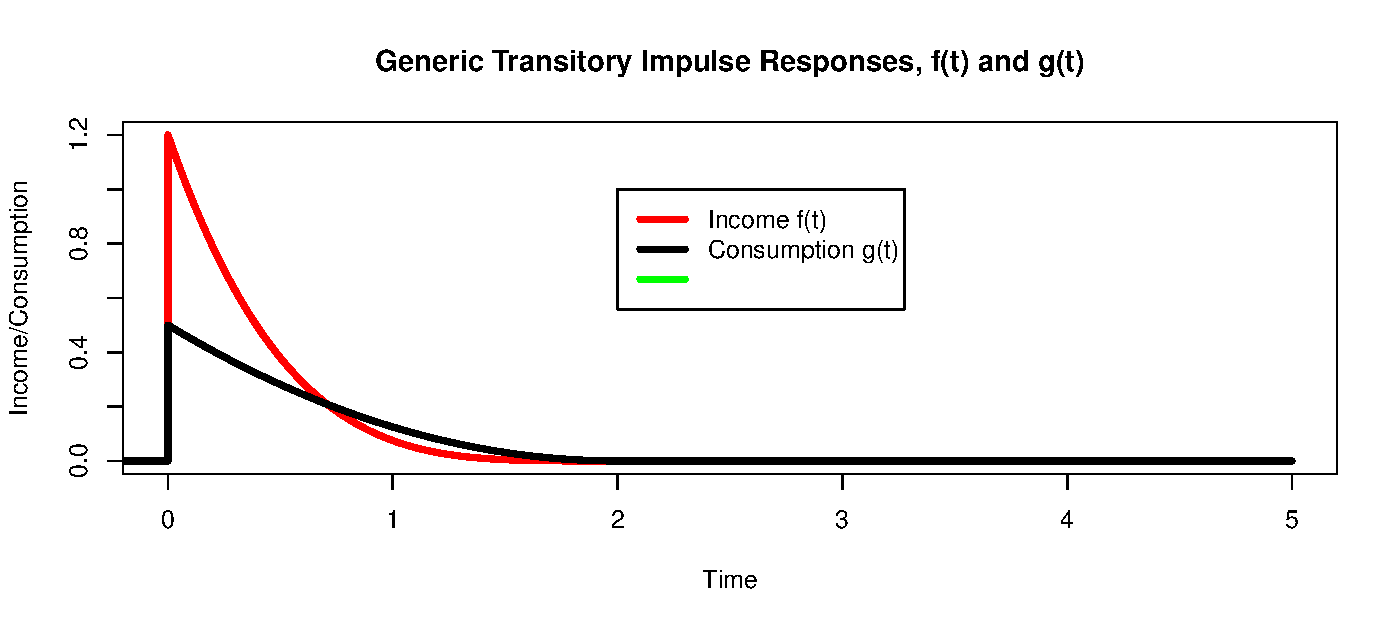
\includegraphics[height=3.5cm]{../Figures/GenericTransitoryConsumption.pdf}};
	\pause
	\node (img2) at (img1) {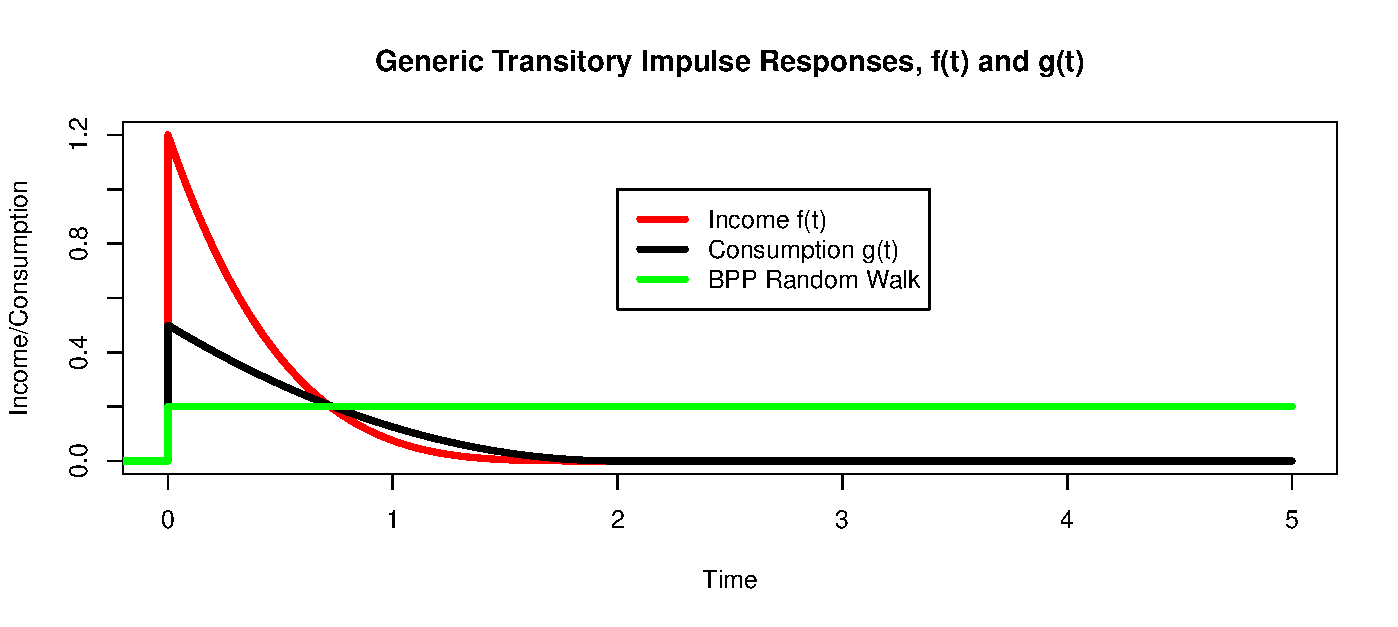
\includegraphics[height=3.5cm]{../Figures/GenericTransitoryConsumptionWithBPP.pdf}};
	\end{tikzpicture}
	\end{center}
	\vspace*{-0.2in}
	This is a key difference between what we assume and BPP
}
\frame
{
	\frametitle{Identification of the Consumption Response}
	Consumption flow is given by:
	\begin{align*}
	c_t  &= \phi p_t  + \int_{t-2}^{t} g(t-s)dq_s  \\
	\implies \mathrm{Cov}(\Delta^N \bar{c_T},\Delta^N \bar{y_T} ) &= \phi (N-\frac{1}{3}) \sigma^2_p + 2 \psi \sigma^2_{\tilde{q}}
	\end{align*}
	where  $\psi = \frac{\mathrm{Cov}(\tilde{c},\tilde{q})}{\mathrm{Var}(\tilde{q})}$, the regression coefficient of `transitory' consumption on transitory income \\
	\pause
	\bigskip
	\begin{itemize}
		\item $\phi$: MPX out of permanent income shocks
		\item $\psi$: MPX out of transitory income shocks
	\end{itemize}
}
\frame
{
	\frametitle{Full Identification}
We use GMM on the equations:
\begin{align*}
\mathrm{Var}(\Delta^N \bar{y_T} ) &=  (N-\frac{1}{3}) \sigma^2_p + 2  \sigma^2_{\tilde{q}} \\
\mathrm{Cov}(\Delta^N \bar{c_T},\Delta^N \bar{y_T} ) &= \phi (N-\frac{1}{3}) \sigma^2_p + 2 \psi \sigma^2_{\tilde{q}}
\end{align*}
with $N=3,4,5$ (total of six equations) to identify the four unknowns:
\begin{itemize}
	\item $\sigma^2_p$: Permanent shock variance
	\item $\sigma^2_{\tilde{q}}$: (Time aggregated) transitory shock variance
	\item $\phi$: MPX out of permanent income shocks
	\item $\psi$: MPX out of transitory income shocks
\end{itemize}
}
\frame
{
	\frametitle{Threats to Identification}
	\begin{minipage}{\textwidth}
		\begin{table}
			\label{table:sourcesofbias}
			\begin{tabular}{lcc}  
				\\ & \multicolumn{2}{c}{\textbf{Direction of Bias} }  
				\\ & Perm MPX & Tran MPX
				\\ \hline
				\\ Persistent Consumption Response & +ve & -ve
				\\ Endogenous Income Shocks & Neutral & +ve
				\\ Income Measurement Error &  Neutral & +ve
				\\ Permanent Shocks are AR(1) & Neutral & +ve
				\\ Non-linear MPX	& ? & ?
				\\ Time-varying risk	& ? & ?
			\end{tabular}
		\end{table}
	\end{minipage}
}
\section{Data}
\frame
{
	\frametitle{Data: Income}
	\begin{itemize}
		\item Starting point: Register based micro data for all Danish households made available by Statistics Denmark
		\item Really good income data
		\begin{itemize}
			\item We use after-tax income for the household head, based on third-party reported tax data
			\item Restrict sample to heads aged 30-55
		\end{itemize}
		\item We divide through by permanent income (mean income over all observed years) and take the residual after controlling for age, education, marital status etc. (along with interactions of these)
	\end{itemize}
}
\frame
{
	\frametitle{Data: Expenditure}
	We use the identity
		\begin{align*}
			C_t \equiv Y_t - S_t = Y_t - P_t - \Delta NW
		\end{align*}
	\begin{itemize}
		\item Deposit and brokerage accounts all third party reported
		\item Works well for households with simple financial lives
		\item Main issue: Capital gains and losses
		\begin{itemize}
			\item Exclude households where methodology will not work well (eg business owners)
			\item Exclude housing wealth and years with housing transactions
			\item Capital gains for stocks based on a diversified index
		\end{itemize}
		\item Noisy, but perhaps better than surveys (Kuchler et al. 2018)
		\item Huge sample size advantage: sample covers 7.6 million observations over 2004-2015
	\end{itemize}
}
\section{MPX by Wealth}
\frame
{
	\frametitle{MPX by Liquid Wealth}
	\label{MPXbyLiquidWealth}
	\begin{columns}
		\column{0.5\linewidth}
		\centering
		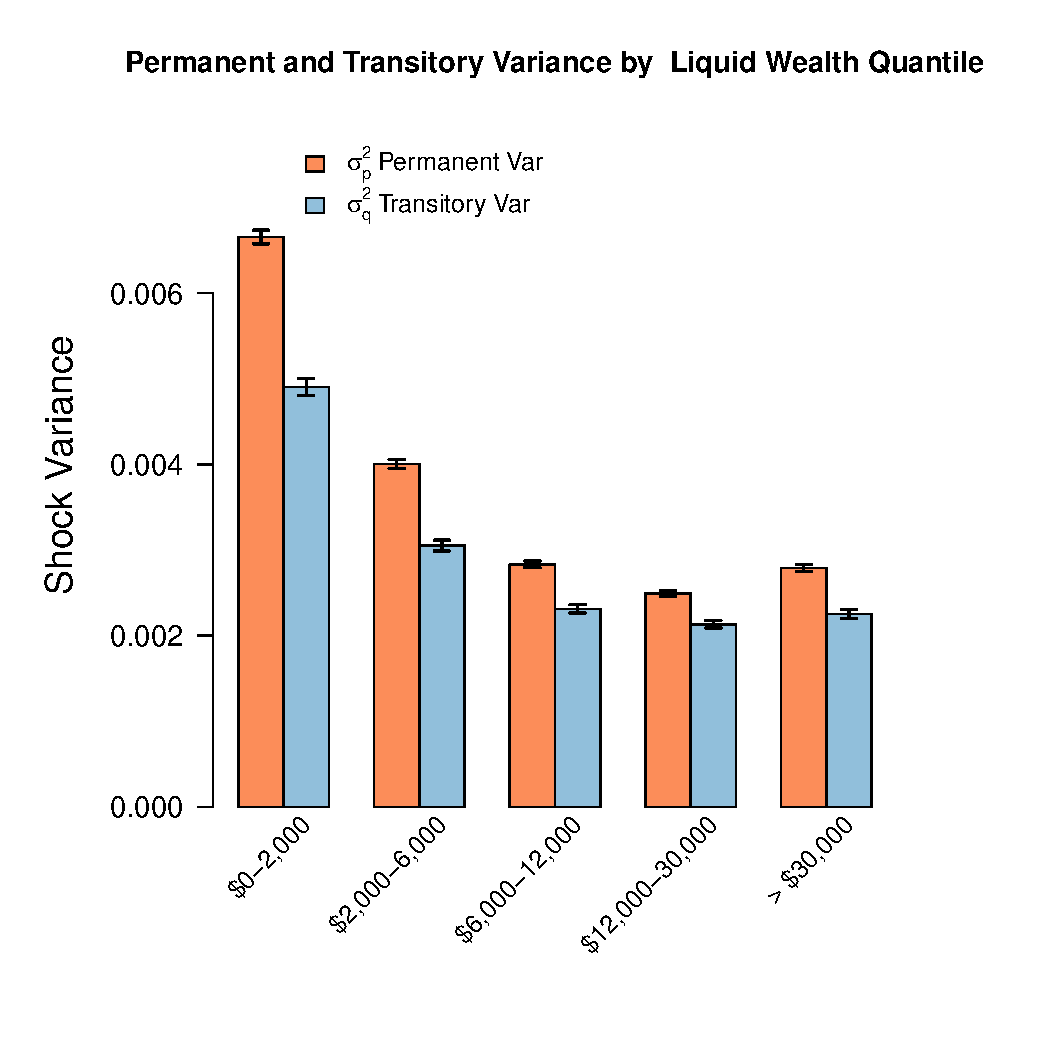
\includegraphics[scale=0.35]{../Figures/VarianceByLiquidWealth_level_lincome_head.pdf}
		\column{0.5\linewidth}
		\centering
		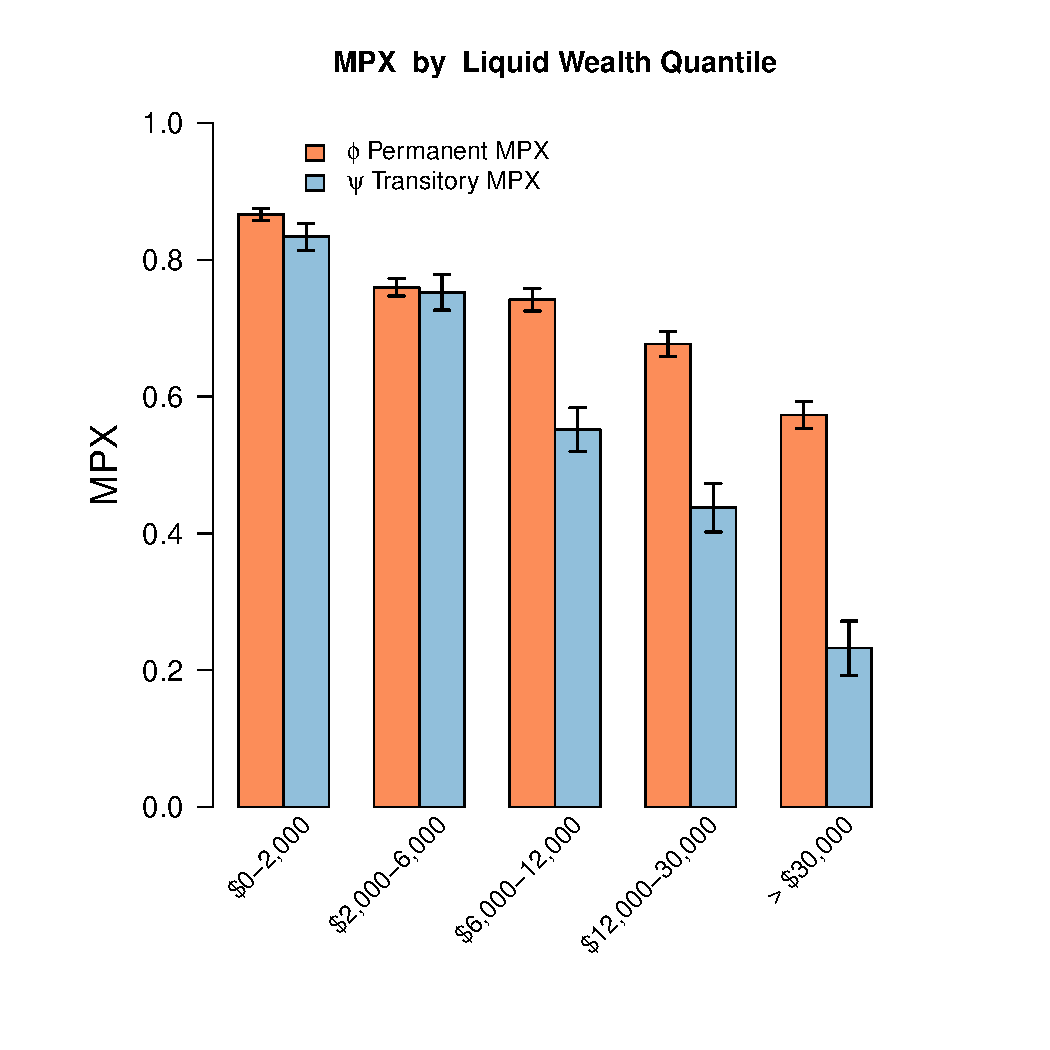
\includegraphics[scale=0.35]{../Figures/MPXByLiquidWealth_level_lincome_head.pdf}
	\end{columns} 
	\hyperlink{MPXbyNetWealth}{\beamerbutton{MPX by Net Wealth}}	
}
\frame
{
	\frametitle{Model vs Data}
	How does a standard model compare with the data?\\
	\begin{columns}
		\column{0.5\linewidth}
		\centering
		\begin{tikzpicture}
		\node (img1) {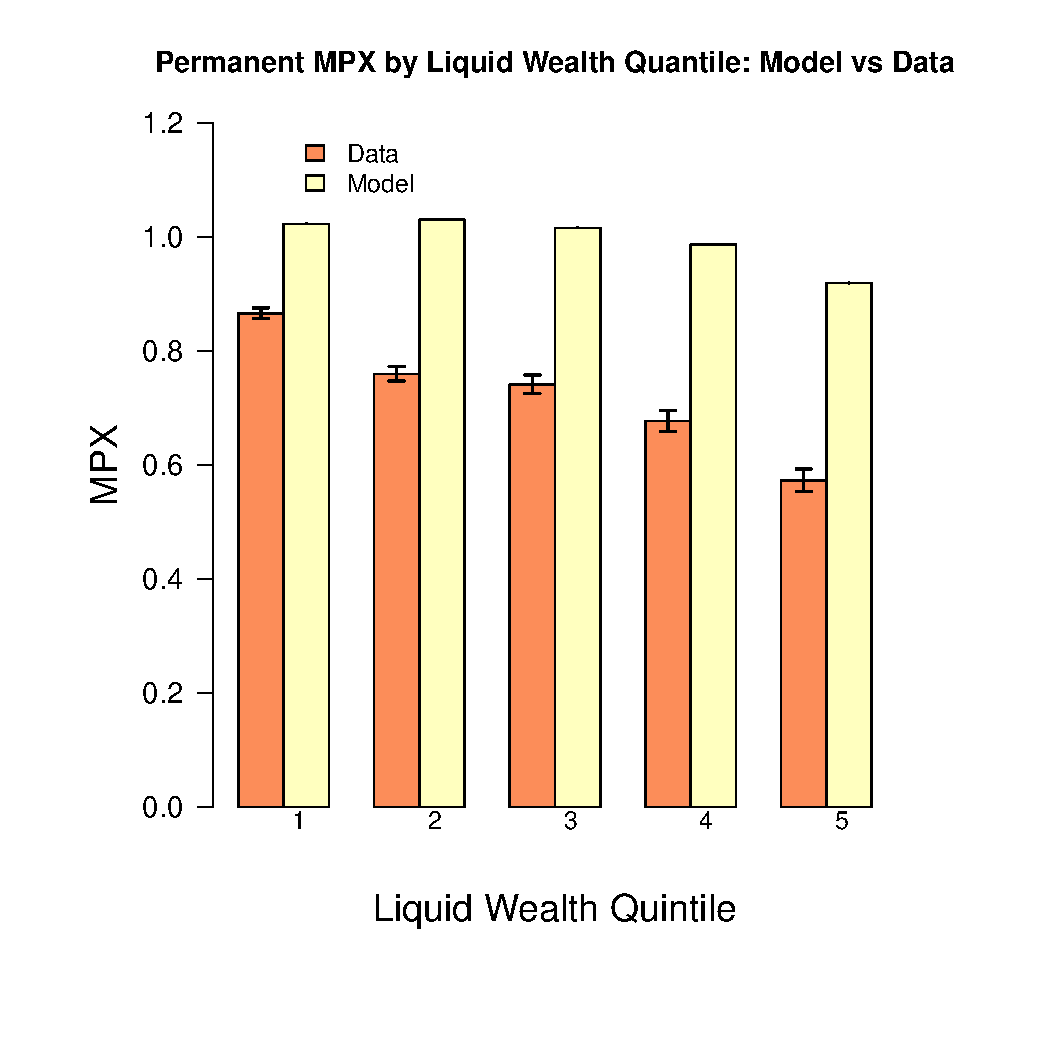
\includegraphics[scale=0.35]{../Figures/benchmark_perm_denmark.pdf}};
		\onslide<2->{
			\node (img2) {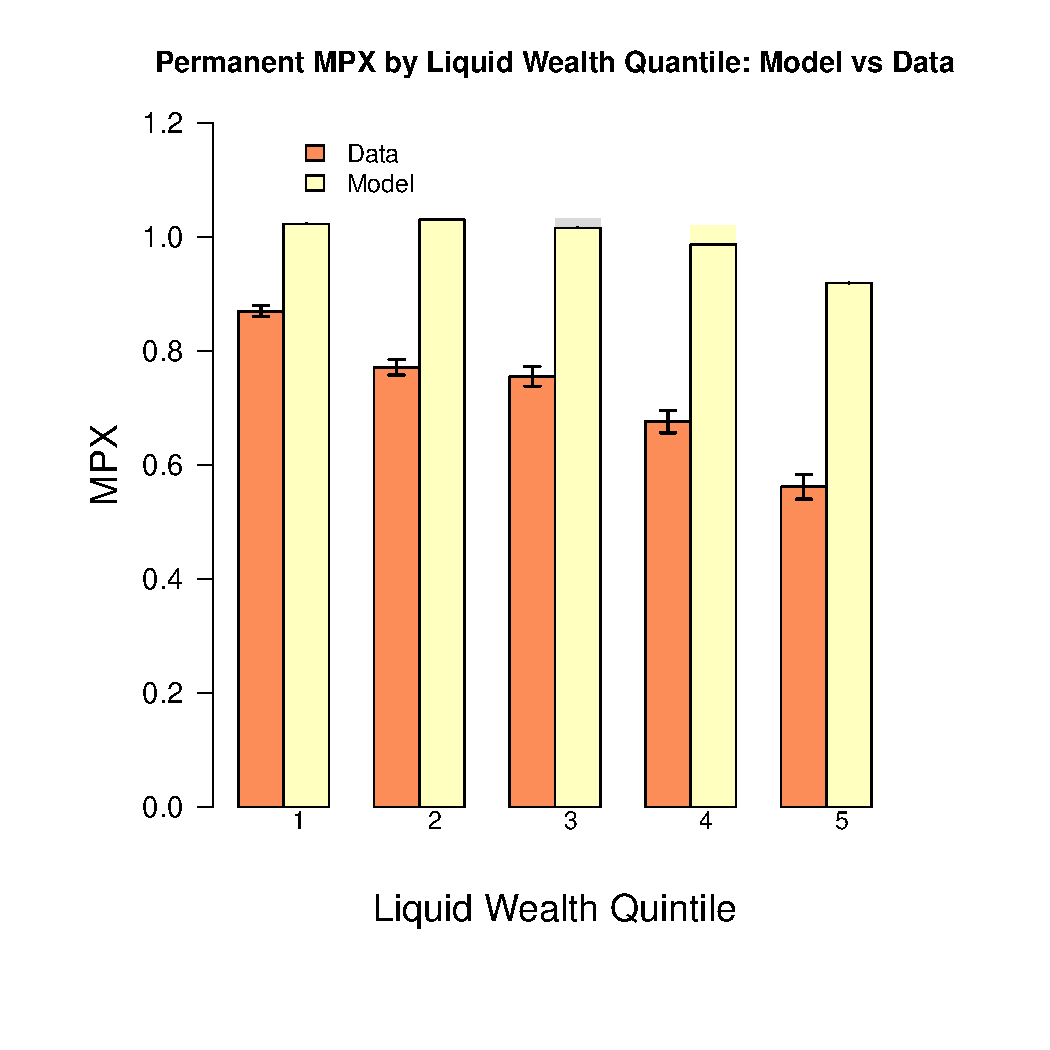
\includegraphics[scale=0.35]{../Figures/prefshock_perm_denmark.pdf}};
		}
		\end{tikzpicture}
		\column{0.5\linewidth}
		\centering
		\begin{tikzpicture}
		\node (img3) {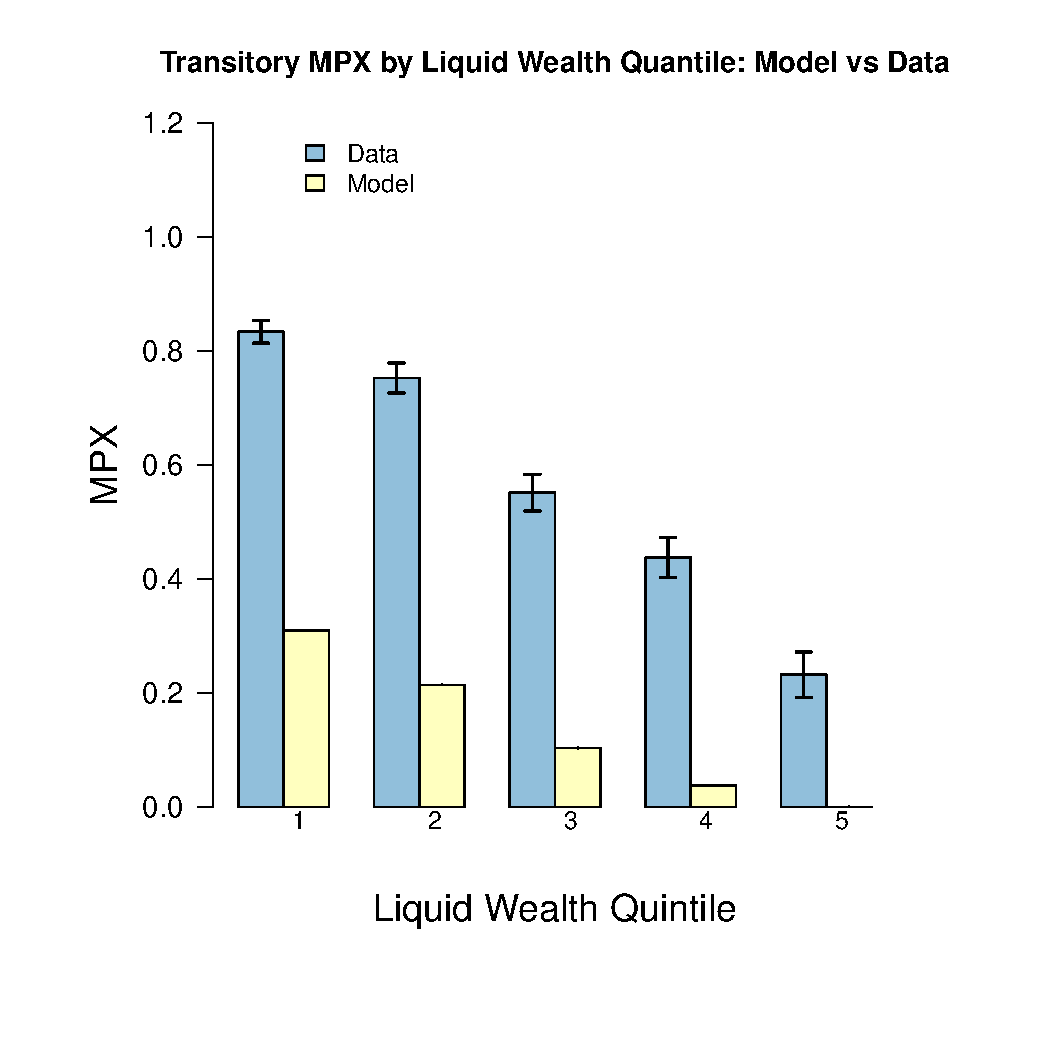
\includegraphics[scale=0.35]{../Figures/benchmark_tran_denmark.pdf}};
		\onslide<2->{
			\node (img4) {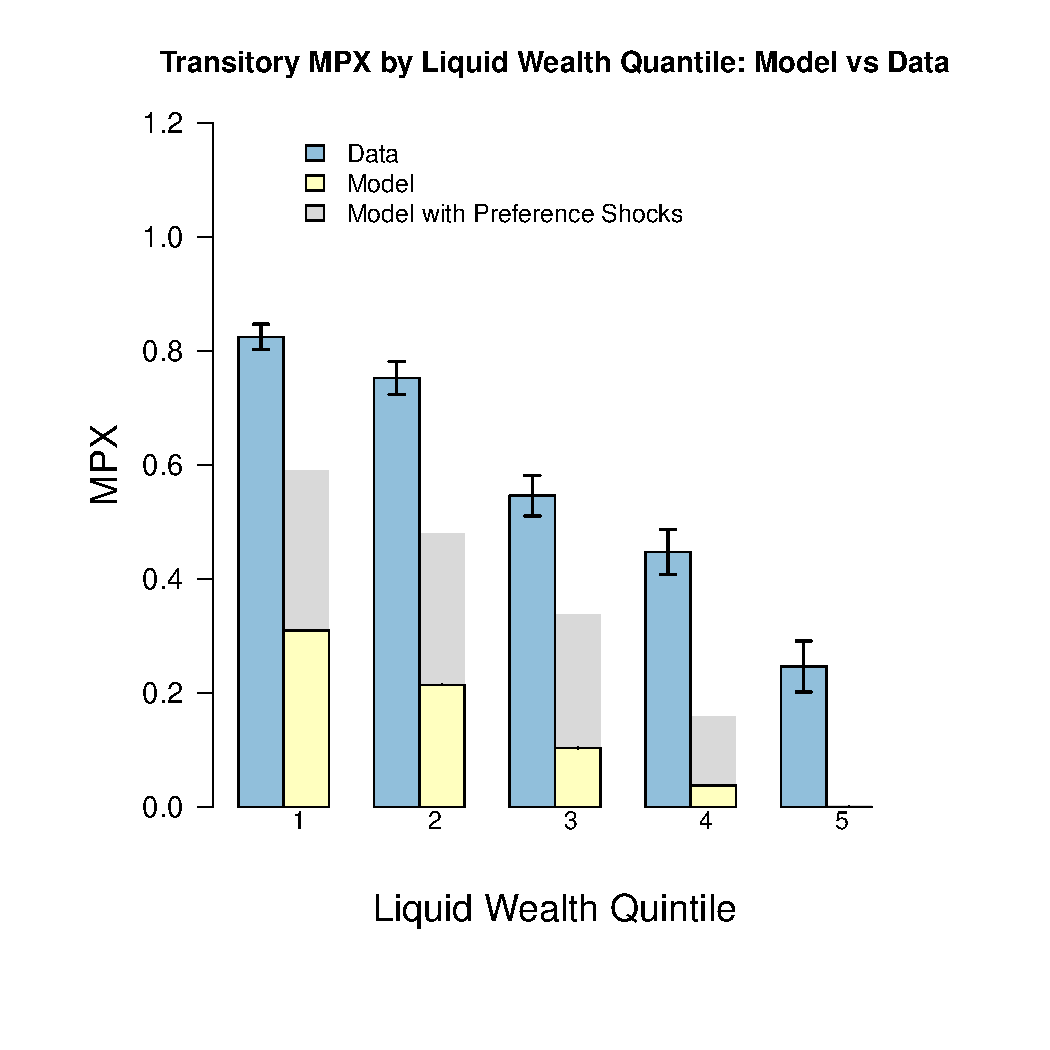
\includegraphics[scale=0.35]{../Figures/prefshock_tran_denmark.pdf}};
		}
		\end{tikzpicture}
	\end{columns} 
}
\section{Application}
\frame{
	\frametitle{Monetary Policy: Measuring Redistribution}
	We calculate the sufficient statistics from \cite{auclert_monetary_2017}\\
	\bigskip
	Here we will focus on the \textit{Interest Rate Exposure} channel:\\
	\bigskip
	If\\
	\begin{itemize}
		\item[1] Households that \textit{owe} a lot of floating rate debt have \textit{high} MPCs\\
		\item[2] Households that \textit{own} a lot of floating rate debt have \textit{low} MPCs
	\end{itemize}
	Then lowering interest rates will on average \textit{increase} consumption through redistribution \\
	\pause
	\bigskip
	Do we know if 1 and 2 hold? How can we measure the size of this effect?
}
\frame{
	\frametitle{Monetary Policy: Measuring Redistribution}
	Define \textit{Unhedged Interest Rate Exposure} for household $i$ as the total savings the household will invest at this year's interest rate:
	\begin{align*}
	URE_i = Y_i - C_i + A_i - L_i
	\end{align*}
	Where
	\begin{itemize}
		\item $Y_i = $ Total after tax income 
		\item $C_i = $ Total Expenditure, including interest payments
		\item $A_i = $ Maturing assets
		\item $L_i = $ Maturing liabilities
	\end{itemize}
	Following a change in the interest rate $dR$, the size of the Interest Rate Exposure channel on household $i$'s expenditure is:
	\begin{align}
		dc_i = MPC_i URE_i  \frac{dR}{R}
	\end{align}
}
\frame{
	\frametitle{Monetary Policy: Measuring Redistribution}
	In aggregate, the size of this channel is given by:
	\begin{align*}
	\frac{dC}{C} &= \mathbb{E}_I \Big(MPC_i \frac{URE_i}{\mathbb{E}_I (c_i)}   \Big) \frac{dR}{R} 
	\end{align*}
	Define sufficient statistic:
	\begin{align*}
	\mathcal{E}_R  = \mathbb{E}_I \Big(MPC_i \frac{URE_i}{\mathbb{E}_I (c_i)}   \Big) 
	\end{align*}
	\bigskip
	$\implies$ Need to know the distribution of $MPC_i$ with $URE_i$\\
	\bigskip
	We can do that!
}
\frame{
	\frametitle{Monetary Policy: Measuring Redistribution}
	\begin{figure}
	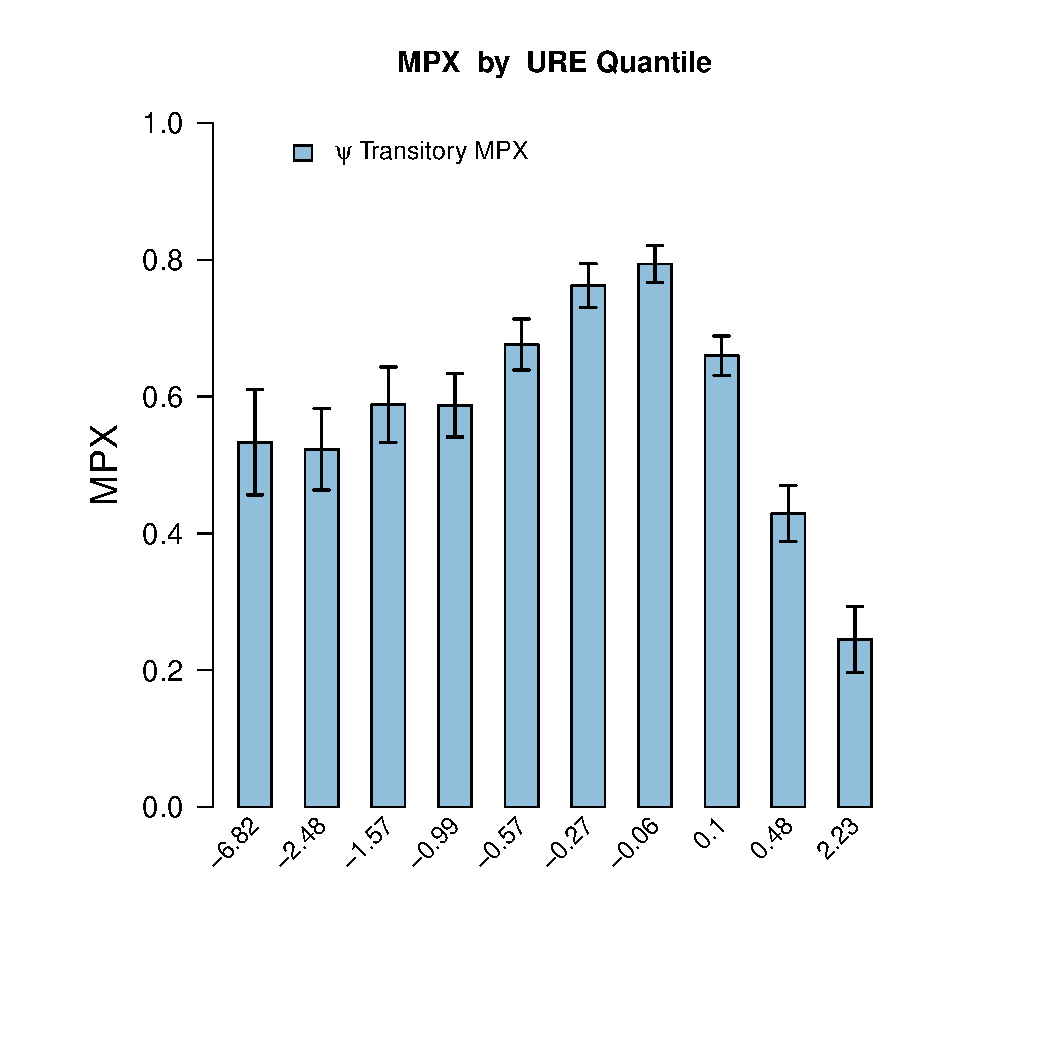
\includegraphics[scale=0.5]{../Figures/MPXByURE_level_lincome_head.pdf}
	\end{figure}
}
\frame{
	\frametitle{Monetary Policy: Measuring Redistribution}
	\textit{Total} URE sums to zero - this is not true for our household sample 
	\begin{itemize} 
		\item -338bn Kr
	\end{itemize}
	\bigskip
	\tiny
	\input ../Tables/URE_table.tex
}
\frame{
	\frametitle{Monetary Policy: Measuring Redistribution}
	The Five Transmission Channels:
	\begin{align*} 
	\frac{dC}{C} &= \overbrace{\mathcal{M}\frac{dY}{Y}}^{\text{Aggregate Income Channel}\qquad} \overbrace{ + \gamma \mathcal{E}_Y \frac{dY}{Y}}^{\text{Earnings Heterogeity Channel}\qquad} \overbrace{ - \mathcal{E}_P\frac{dP}{P}}^{\text{Fisher Channel}}  \nonumber \\
	& \qquad \underbrace{ + \mathcal{E}_R \frac{dR}{R}}_{\text{Interest Rate Exposure Channel}\qquad}  \underbrace{ - \sigma \mathcal{S}\frac{dR}{R}}_{\text{Intertemporal Substitution Channel}} \label{auclert_channels}
	\end{align*}
	\pause
	\begin{columns}
	\column{0.5\linewidth}
	\centering
		\input ../Tables/sufficient_stats2.tex
	\column{0.5\linewidth}
	\pause
	Compare $\mathcal{E}_R$ to $\sigma S$: \\
	\bigskip
	$\sigma$ in the range of 0.1 to 0.5 (maybe) \\
	\bigskip
	 $\sigma S \approx 0.06 - 0.28$ \\
	\end{columns}
}
\section{MPC vs MPX}
\frame
{
	\frametitle{Durables}
	We have data on value of household cars\\
	\begin{itemize}
		\item Construct expenditure excluding car purchases and sales
		\begin{align*}
		C_T^{\text{nocar}} = C_T - \Delta \text{CarValue}
		\end{align*}
		\item Construct proxy for non durable consumption (Cars $\approx 42.1\%$ durable expenditure)
		\begin{align*}
		C_T^{\text{nondurable}} = C_T - \frac{1}{0.421}\Delta \text{CarValue}
		\end{align*}
	\end{itemize}
}
\frame
{
	\frametitle{Durables}
	\begin{center}
		\begin{tikzpicture}
		\node (img1) {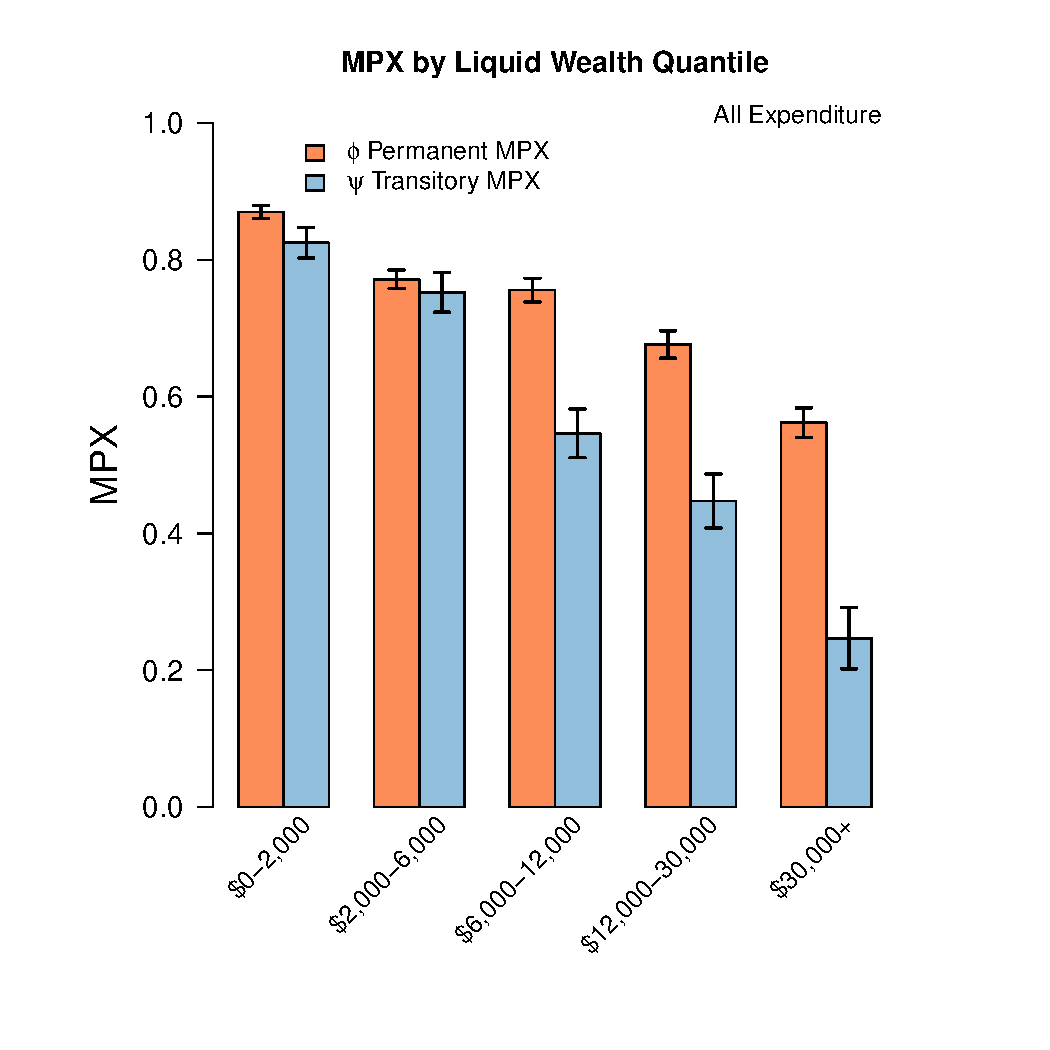
\includegraphics[scale=0.4]{../Figures/MPXByDurables_all.pdf}};
		\pause
		\node (img2)
		{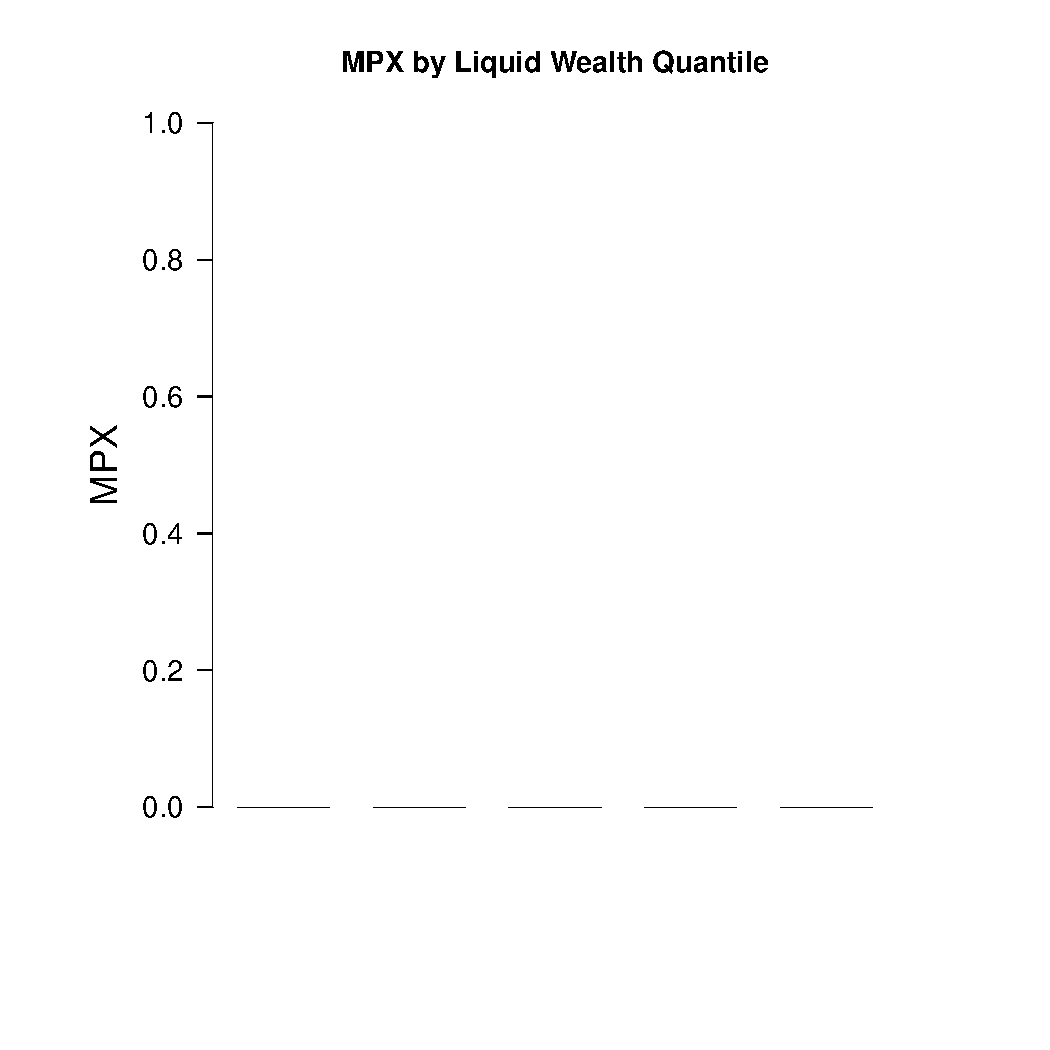
\includegraphics[scale=0.4]{../Figures/MPXByDurables_blank.pdf}};
		\node (img3) {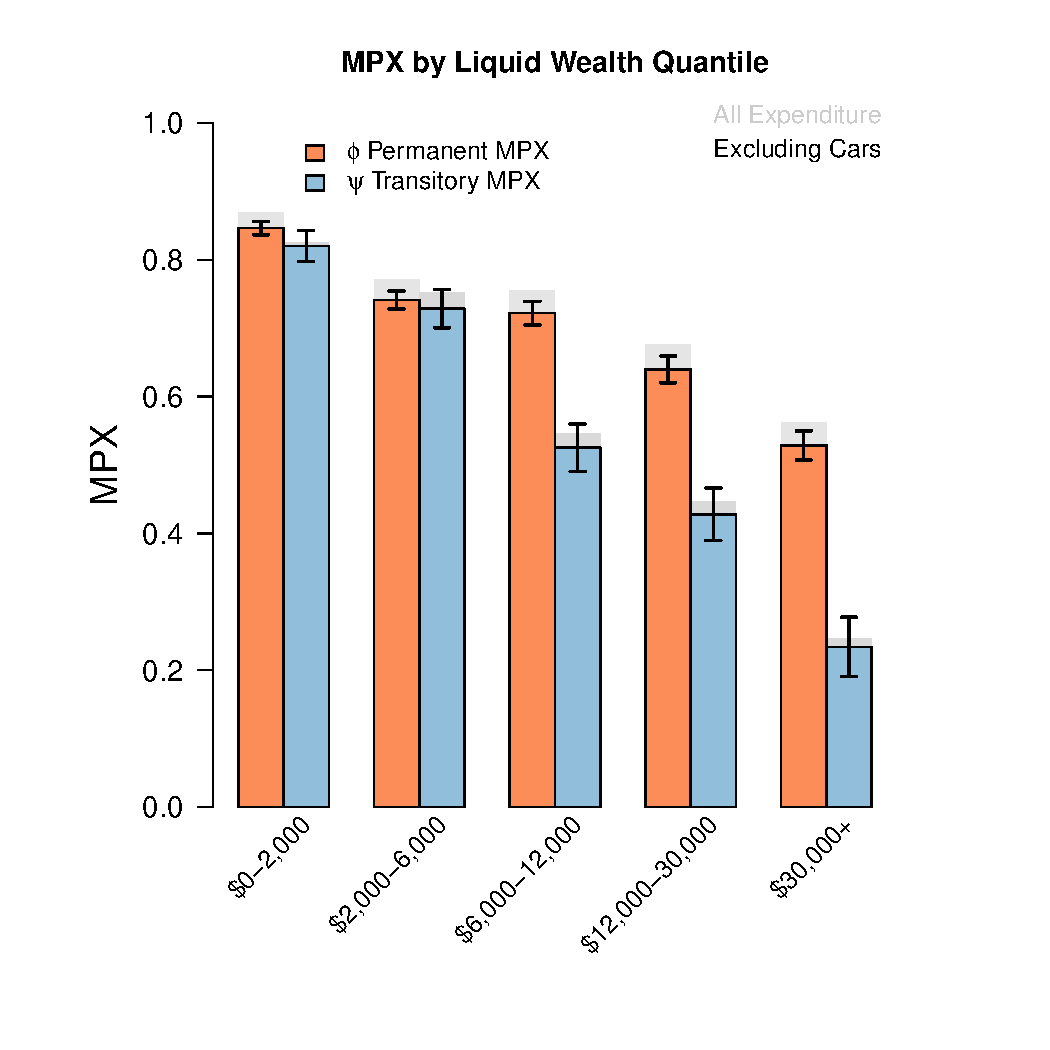
\includegraphics[scale=0.4]{../Figures/MPXByDurables_nocar.pdf}};
		\pause
		\node (img4)
		{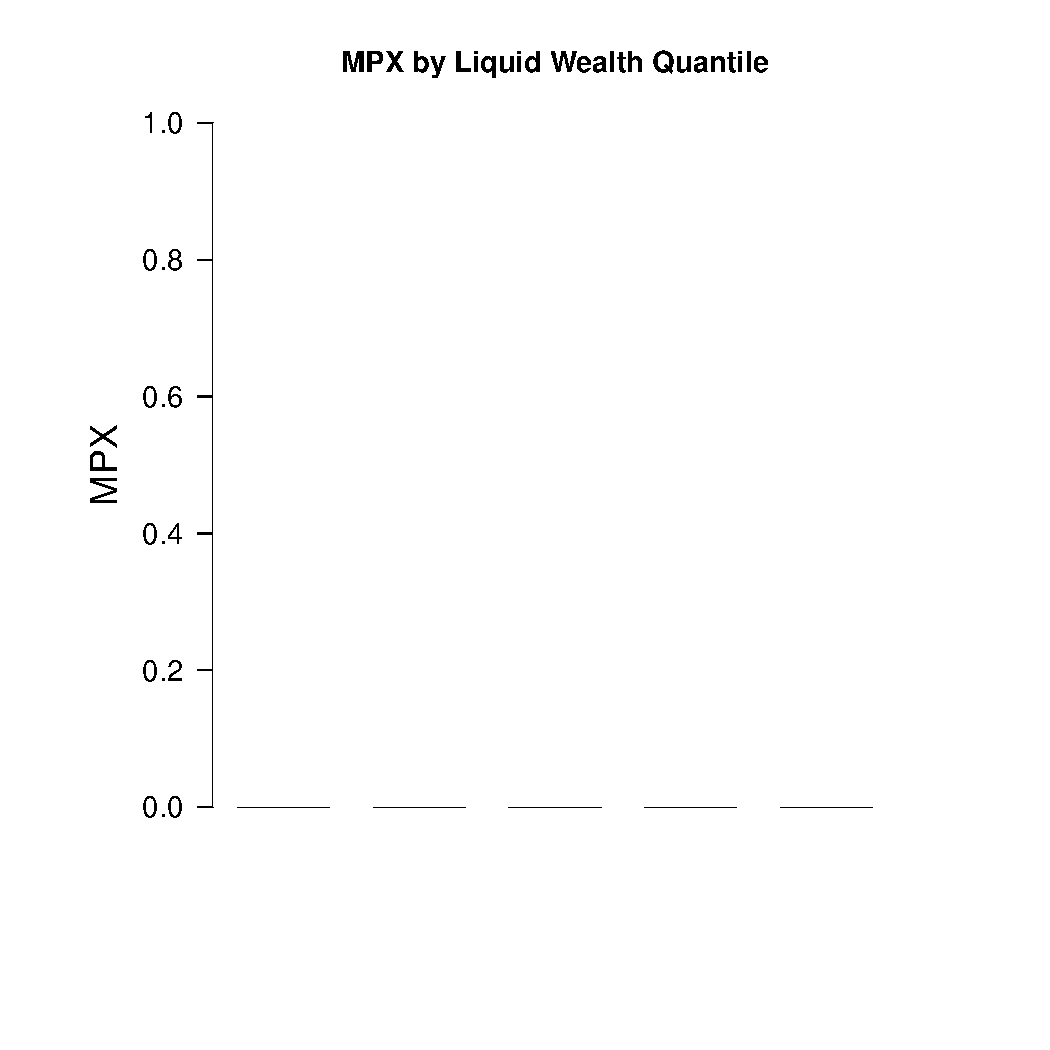
\includegraphics[scale=0.4]{../Figures/MPXByDurables_blank.pdf}};
		\node (img5) {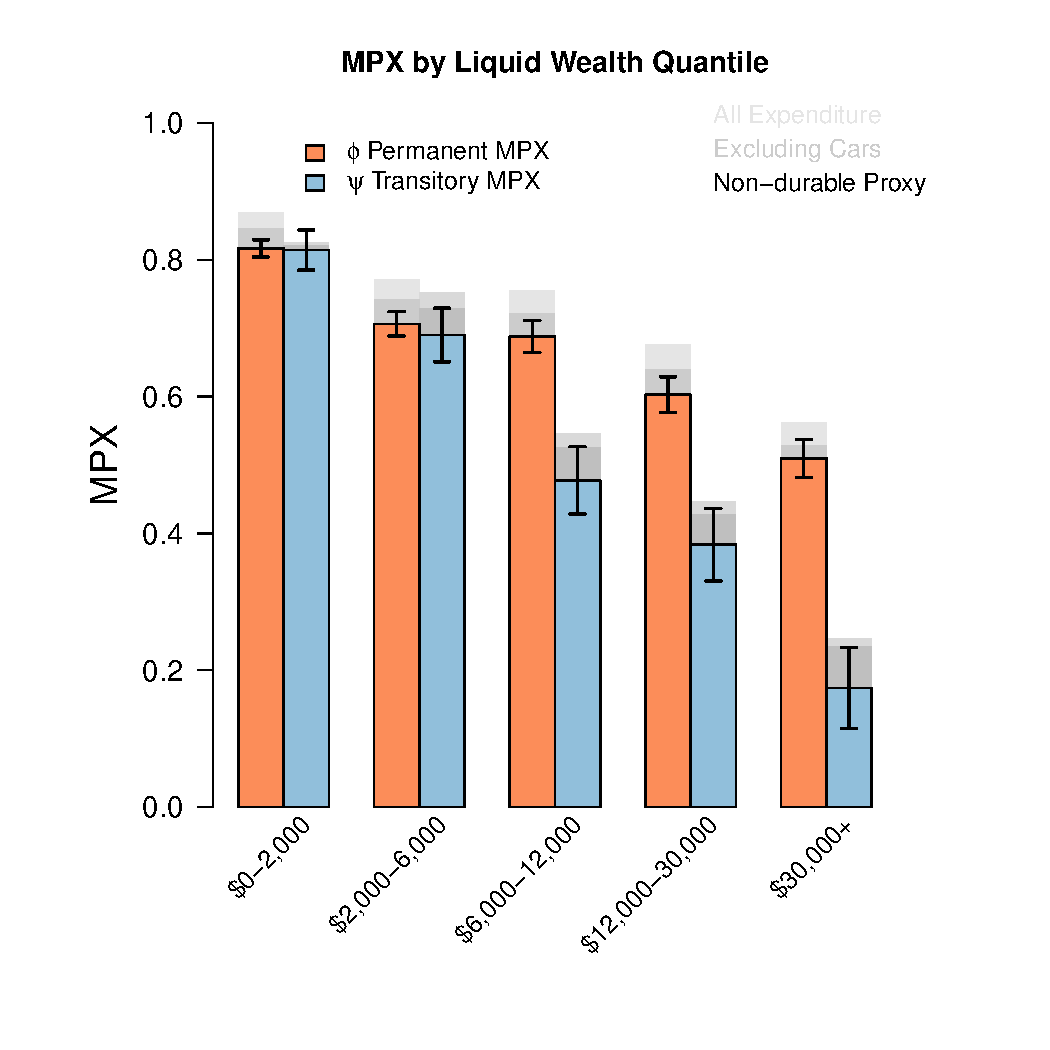
\includegraphics[scale=0.4]{../Figures/MPXByDurables_nodurableproxy.pdf}};
		\end{tikzpicture}
	\end{center}
}
\section{Conclusion}
\frame{
	\frametitle{Conclusion}
	\begin{itemize}
		\item We have designed a new method to estimate consumption responses to income shocks
		\item It appears to work well, both in theory and practice
		\item We can use it to show that heterogeneity plays a key role in monetary policy transmission
	\end{itemize}
	\bigskip
	Thank you!
}
\appendix
\section{Appendix}
\frame{
	\frametitle{Evidence of Consumption Decay Within 2 Years}
	\label{cons_decay}
	\begin{columns}
	\column{0.35\linewidth}
	\begin{figure}
	From \cite{fagereng_mpc_2016}
	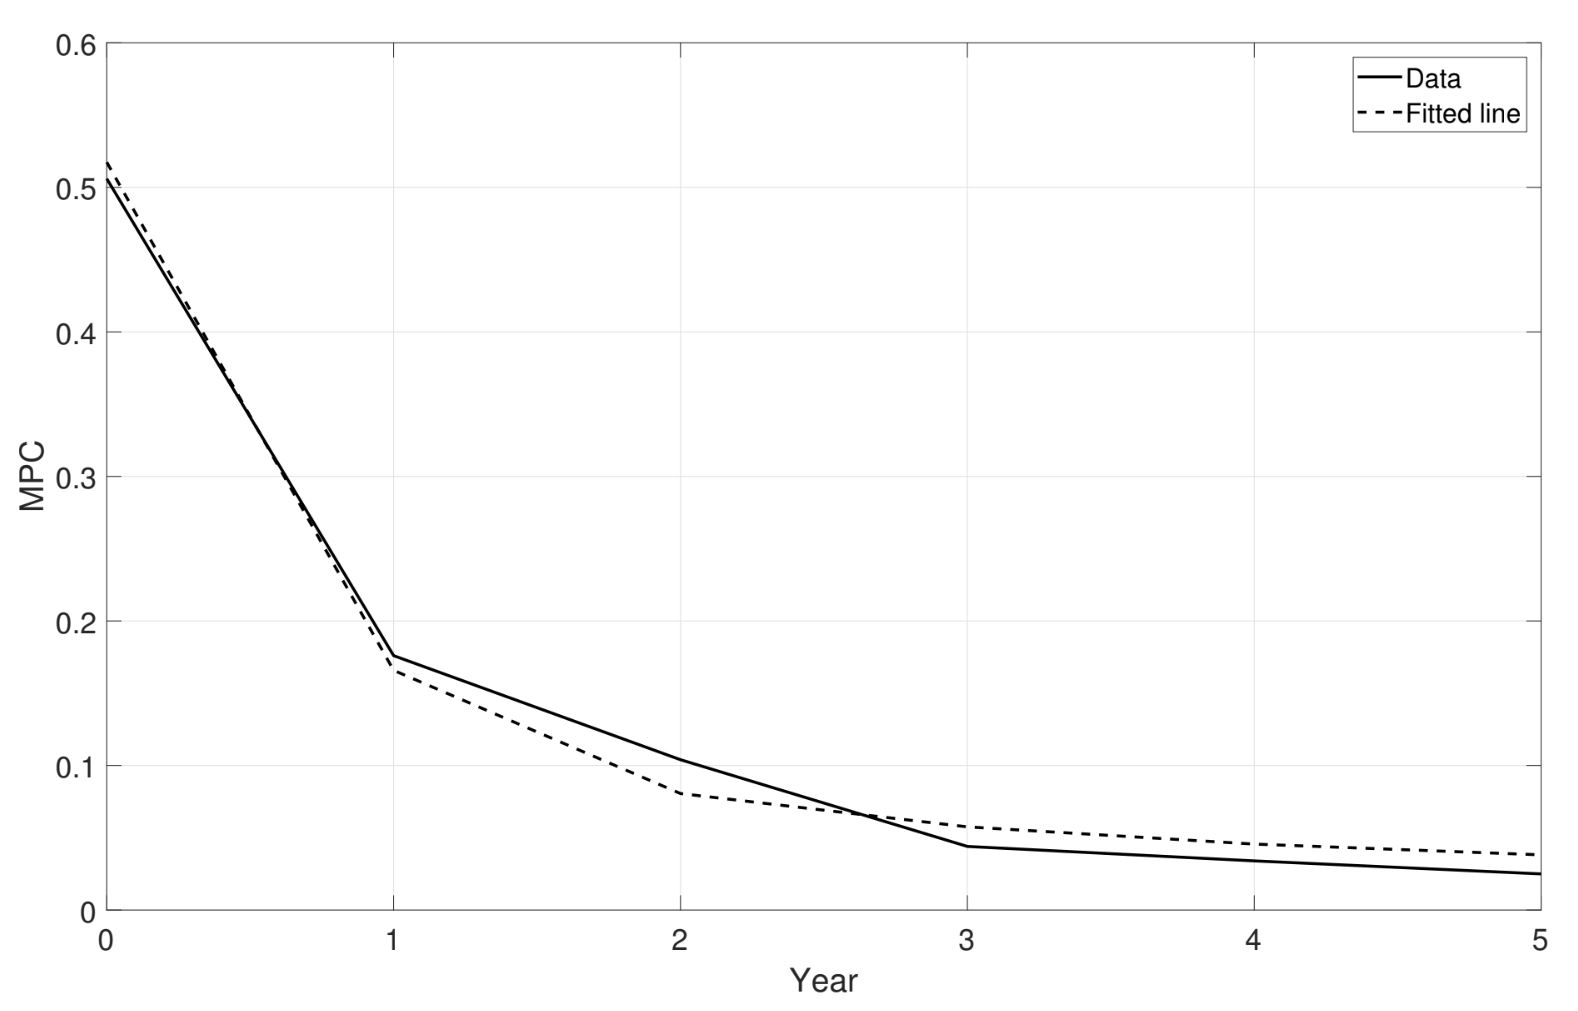
\includegraphics[scale=0.3]{../Figures/norway_cons_decay.jpg}
	\end{figure}
	\column{0.5\linewidth}
	\begin{figure}
	From \cite{gelman_what_2016}
	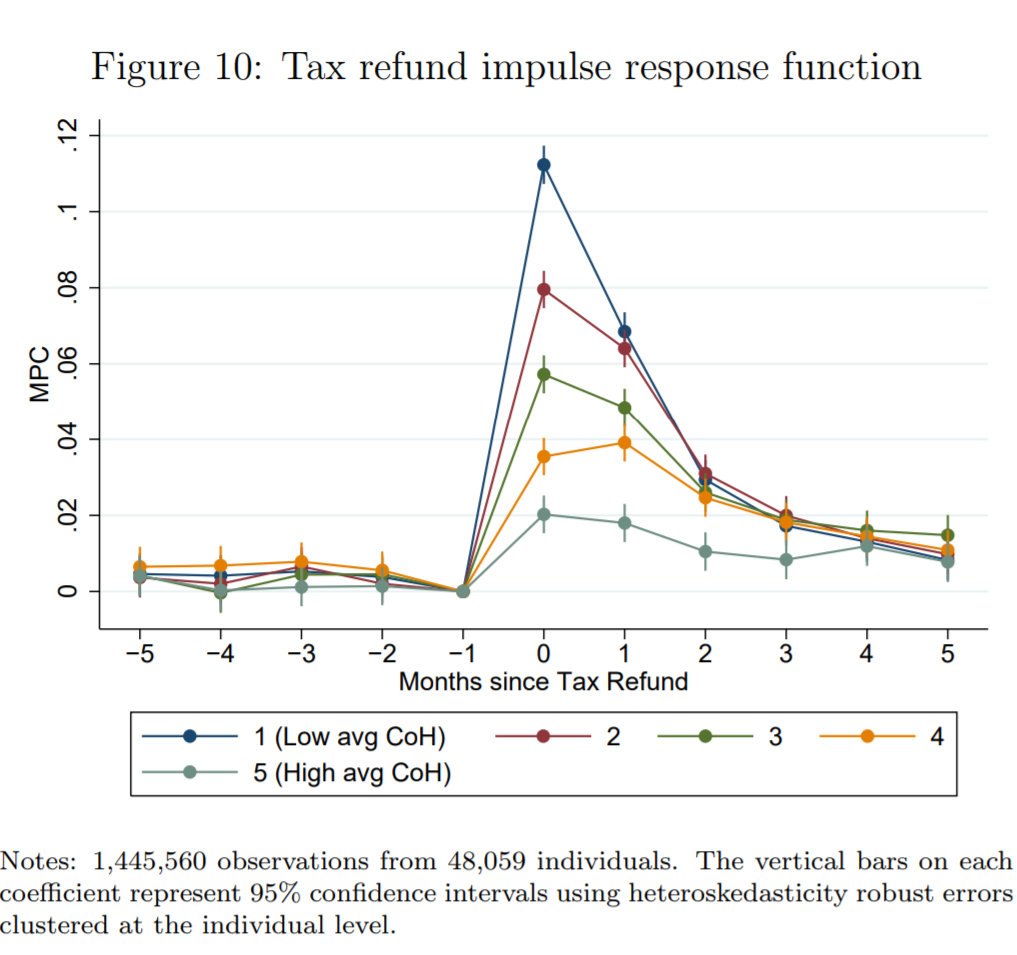
\includegraphics[scale=0.1]{../Figures/gelman_cons_decay.png}
	\end{figure}
	\end{columns}
	\hyperlink{cons_identification}{\beamerbutton{Back}}
}
\frame
{
	\frametitle{MPX by Net Wealth}
	\label{MPXbyNetWealth}
	\begin{columns}
		\column{0.5\linewidth}
		\centering
		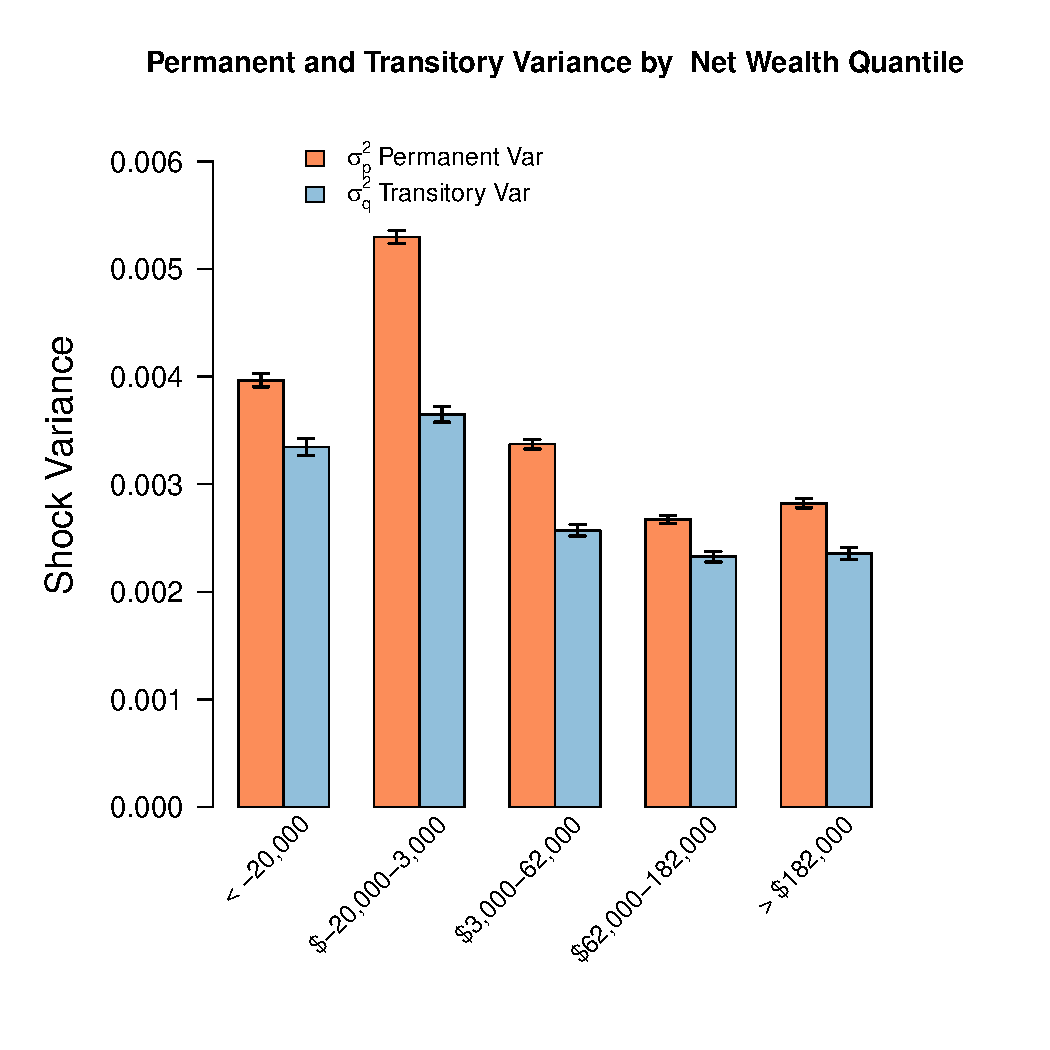
\includegraphics[scale=0.35]{../Figures/VarianceByNetWealth_level_lincome_head.pdf}
		\column{0.5\linewidth}
		\centering
		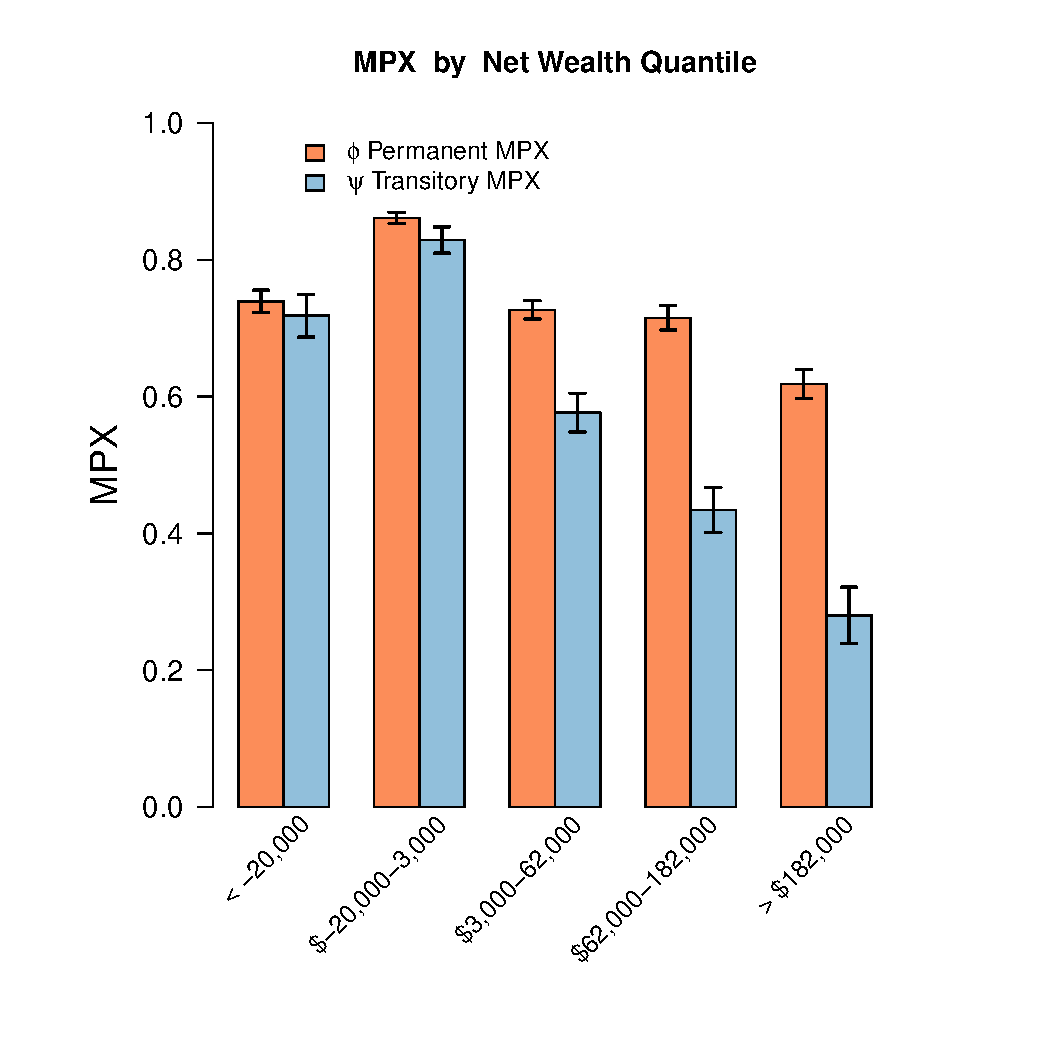
\includegraphics[scale=0.35]{../Figures/MPXByNetWealth_level_lincome_head.pdf}
	\end{columns} 	
	\hyperlink{MPXbyLiquidWealth}{\beamerbutton{Back}}
}
\begin{comment}
\section{Model}
\frame
{
	\frametitle{Model}
	How does this compare with a standard buffer-stock saving model?
	\begin{itemize}
		\item Build model to match Danish income process
		\item Allow \textit{heterogeneous discount factors} in order to match the distribution of \textit{liquid} assets in Denmark
		\item See how the distribution of transitory MPX varies with liquid asset holdings
	\end{itemize}
}
\frame
{
	\frametitle{Model}
Given market resources ($\boldmath{\mLevBF}_t$), households in this model maximize expected utility:
\begin{align*}
\mathbb{E}_t \sum_{i=t}^{\infty} \beta^i(1-D)^i  u(\cLevBF_i)
\end{align*}
subject to the constraints:
\begin{align*}
\aLevBF_t = \mLevBF_t - \cLevBF_t \\
\bLevBF_t = R\aLevBF_t \\
\yLevBF_t = \theta_t \pLevBF_t \\
\pLevBF_t = \Psi_t \pLevBF_{t-1} \\
\mLevBF_t = \bLevBF_t + \yLevBF_t
\end{align*}
}
\frame
{
	\frametitle{Calibration}
	\input ../Tables/CalibrationTable.tex
}
\frame
{
	\frametitle{Lorenz Curve}
	Lorenz Curve for Liquid Wealth Holdings
	\centering
	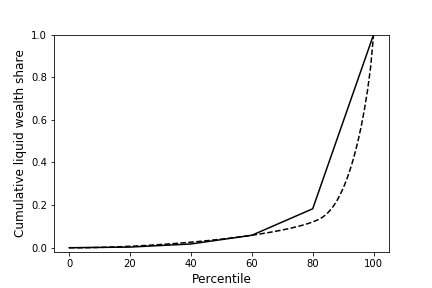
\includegraphics[scale=0.5]{../Figures/Lorenz.png}
}
\frame
{
	\frametitle{Does our Methodology Work?}
	\begin{columns}
	\column{0.5\linewidth}
	\centering
	
\includegraphics[scale=0.35]{../Figures/MPC_accuracy.png}
	\column{0.5\linewidth}
	\begin{itemize}
		\item Estimate is larger than 6m MPX for low liquid wealth
		\begin{itemize}
		\item Income jumps can be large
		\end{itemize}
		\item Estimate is smaller than 6m MPX for high levels of wealth
		\begin{itemize}
		\item Consumption response lasts more than 2 years
		\end{itemize}
	\end{itemize}
	\end{columns}
}
\frame
{
	\frametitle{Model vs Data}
	How does the model compare with the data?
	\begin{columns}
	\column{0.5\linewidth}
	\centering
	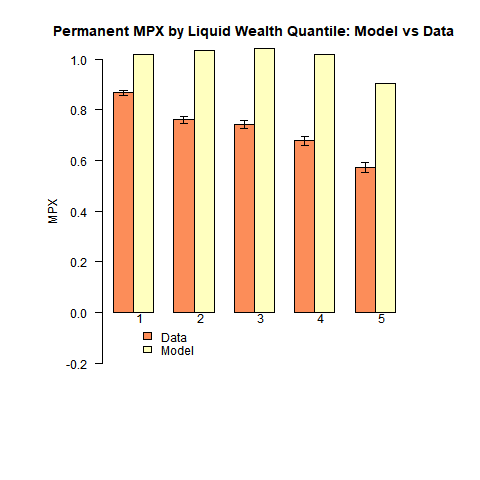
\includegraphics[scale=0.35]{../Figures/CSTW_perm_denmark.png}
	\column{0.5\linewidth}
	\centering
	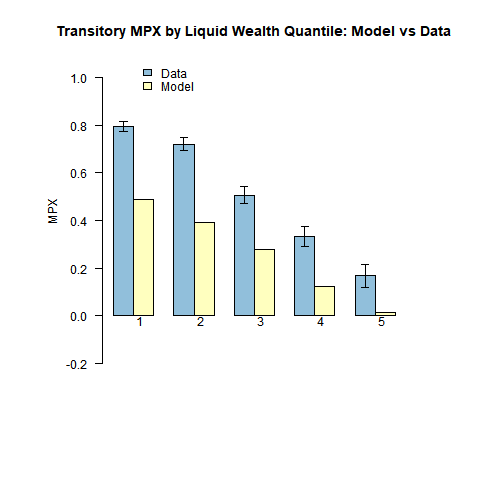
\includegraphics[scale=0.35]{../Figures/CSTW_tran_denmark.png}
	\end{columns} 
}
\section{Threats to Identification}
\frame
{
	\frametitle{Endogenous Income Shocks}
	\begin{itemize}
		\item Household's consumption preference highly variable
		\item Hours worked is endogenous
	\end{itemize}
	The household maximizes:
	\begin{align*}
	\mathbb{E}_t \sum_{n=t}^{\infty} \beta^n \Bigg(\mathcal{X}_n \frac{ \cLevBF_n^{1-\rho}}{1-\rho}-\frac{\lLevBF_n^{1+\frac{1}{\xi}}}{1+\frac{1}{\xi}} \Bigg)
	\end{align*}
	\begin{itemize}
	\item Frisch elasticity $\xi$ 
	\item Preference shock $\mathcal{X}$
	\end{itemize}
}
\frame
{
	\frametitle{Endogenous Income Shocks}
	\input ../Tables/experimental/mpc_laborsupply.tex \\
	\input ../Tables/experimental/psi_laborsupply.tex
}
\frame
{
	\frametitle{Persistent Consumption Response}
	We assume the transitory consumption response lasts less than 2 years \\
	\begin{columns}
	\column{0.5\linewidth}
	\centering 
		High MPC Model\\
	\input ../Tables/experimental/Psi_array1.tex 
	\column{0.5\linewidth}
	\centering
	Low MPC Model\\
	\input ../Tables/experimental/Psi_array2.tex
\end{columns} 
	When MPCs are low, this assumption does not hold in the model, leading to downward bias		
}
\frame
{
	\frametitle{Income Measurement Error}
	Imputation method means measurement error in income shows up in consumption too\\
	Example:
	\begin{itemize}
		\item Actual transitory MPX is zero
		\item 25\% of transitory income variance is due to measurement error
		\item Methodology would result in MPX estimate of 25\%
	\end{itemize}	
	\pause
	But:
	\begin{itemize}
	\item Income is well measured (administrative data)
	\item Bias is much larger for households with small MPCs
	\begin{itemize}
		\item MPX for high liquid wealth households is close to zero
	\end{itemize}
\end{itemize}
}
\frame
{
	\frametitle{Permanent Shocks are AR(1)}
	How does our methodology do if permanent income follows an AR(1) process?
	\begin{align*}
	p_{t} = \rho p_{t-1} + \varepsilon_{t} \\
	y_t = p_t + q_t \\
	c_{t} = \phi y_t + \psi q_t
	\end{align*}
	\centering	
	\input ../Tables/experimental/psi_AR1.tex
}


%%%%%%%%%%%%%%%  bibliography
%%%%%%%%%%%%%%%%%%%%%%%%%%%%%%%%%%%%%%%%%%%%%%%%%%%%%%%%%%%%%%%%%%%%%%%%%%%%%%%%%%%%%%%%%%%%%%%%%%%%%%%%%%%%%%
\tiny

\beamerdefaultoverlayspecification{<*>}
\section{}

\begin{frame}[t,allowframebreaks]
	\frametitle{References}
	
	\bibliographystyle{econtex}
	\bibliography{../AllPapers}
\end{frame}

\normalsize
\end{comment}
\bibliographystyle{econtex}
\newsavebox\mytempbib
\savebox\mytempbib{\parbox{\textwidth}{\bibliography{../AllPapers}}}


\end{document}


